\documentclass[11pt,a4paper,dvipsnames]{article}
\usepackage[margin=2.5cm]{geometry}
\usepackage[local]{gitinfo2}
\usepackage{iohk}
\usepackage{microtype}
\usepackage{mathpazo} % nice fonts
\usepackage{amsmath}
\usepackage{amssymb}
\usepackage{amsthm}
\usepackage{latexsym}
\usepackage{mathtools}
\usepackage{stmaryrd}
\usepackage{extarrows}
\usepackage{slashed}
\usepackage[colon]{natbib}
\usepackage[unicode=true,pdftex,pdfa,colorlinks=true]{hyperref}
\usepackage{xcolor}
\usepackage[capitalise,noabbrev,nameinlink]{cleveref}
\usepackage{float}
\floatstyle{boxed}
\restylefloat{figure}
\usepackage{tikz}

%%
%% Package `semantic` can be used for writing inference rules.
%%
\usepackage{semantic}
%% Setup for the semantic package
\setpremisesspace{20pt}

%%
%% Types
%%
\newcommand{\N}{\ensuremath{\mathbb{N}}}
\newcommand{\Npos}{\ensuremath{\mathbb{N}^{+}}}
\newcommand{\Z}{\ensuremath{\mathbb{Z}}}
\newcommand{\R}{\ensuremath{\mathbb{R}}}
\newcommand{\Rnn}{\ensuremath{\mathbb{R}^{\geq 0}}}
\newcommand{\Tx}{\type{Tx}}
\newcommand{\TxBody}{\type{TxBody}}
\newcommand{\Ix}{\type{Ix}}
\newcommand{\TxId}{\type{TxId}}
\newcommand{\Addr}{\type{Addr}}
\newcommand{\UTxO}{\type{UTxO}}
\newcommand{\Wdrl}{\type{Wdrl}}
\newcommand{\Value}{\type{Value}}
\newcommand{\Coin}{\type{Coin}}
\newcommand{\PParams}{\type{PParams}}
\newcommand{\Slot}{\type{Slot}}
\newcommand{\Duration}{\type{Duration}}
\newcommand{\StakePools}{\type{StakePools}}
\newcommand{\StakeKeys}{\type{StakeKeys}}

\newcommand{\DCert}{\type{DCert}}
\newcommand{\DCertRegKey}{\type{DCert_{regkey}}}
\newcommand{\DCertDeRegKey}{\type{DCert_{deregkey}}}
\newcommand{\DCertDeleg}{\type{DCert_{delegate}}}
\newcommand{\DCertRegPool}{\type{DCert_{regpool}}}
\newcommand{\DCertRetirePool}{\type{DCert_{retirepool}}}
\newcommand{\PoolParam}{\type{PoolParam}}
\newcommand{\UTxOState}{\ensuremath{\type{UTxOState}}}
\newcommand{\ledgerState}{\ensuremath{\type{ledgerState}}}

\newcommand{\AddrRWD}{\type{Addr_{rwd}}}
\newcommand{\AddrB}{\type{Addr_{base}}}
\newcommand{\AddrP}{\type{Addr_{ptr}}}
\newcommand{\AddrE}{\type{Addr_{enterprise}}}
\newcommand{\Ptr}{\type{Ptr}}
\newcommand{\DState}{\type{DState}}
\newcommand{\DWEnv}{\type{DWEnv}}
\newcommand{\DPSEnv}{\type{DPSEnv}}
\newcommand{\DPEnv}{\type{DPEnv}}
\newcommand{\DEnv}{\type{DEnv}}
\newcommand{\PEnv}{\type{PEnv}}
\newcommand{\DPState}{\type{DPState}}
\newcommand{\PState}{\type{PState}}
\newcommand{\DCertBody}{\type{DCertBody}}
\newcommand{\TData}{\type{TData}}
\newcommand{\DPoolReap}{\ensuremath{\type{poolreap}}}

%% Adding witnesses
\newcommand{\TxIn}{\type{TxIn}}
\newcommand{\TxOut}{\type{TxOut}}
\newcommand{\VKey}{\type{VKey}}
\newcommand{\SKey}{\type{SKey}}
\newcommand{\HashKey}{\type{HashKey}}
\newcommand{\KeyPair}{\type{KeyPair}}
\newcommand{\Sig}{\type{Sig}}
\newcommand{\Data}{\type{Data}}
%% Adding delegation
\newcommand{\Epoch}{\type{Epoch}}
\newcommand{\VKeyGen}{\type{VKeyGen}}
%% Blockchain
\newcommand{\Gkeys}{\var{G_{keys}}}
\newcommand{\Block}{\type{Block}}
\newcommand{\SlotId}{\type{SlotId}}
\newcommand{\UTxOEnv}{\type{UTxOEnv}}
\newcommand{\CEEnv}{\type{CEEnv}}
\newcommand{\CEState}{\type{CEState}}
\newcommand{\BDEnv}{\type{BDEnv}}
\newcommand{\BDState}{\type{BDState}}
\newcommand{\LEnv}{\type{LEnv}}
\newcommand{\LState}{\type{LState}}

%%
%% Functions
%%
\newcommand{\txins}[1]{\fun{txins}~ \var{#1}}
\newcommand{\txouts}[1]{\fun{txouts}~ \var{#1}}
\newcommand{\txcerts}[1]{\fun{txcerts}~ \var{#1}}
\newcommand{\txid}[1]{\fun{txid}~ \var{#1}}
\newcommand{\outs}[1]{\fun{outs}~ \var{#1}}
\newcommand{\values}[1]{\fun{values}~ #1}
\newcommand{\balance}[1]{\fun{balance}~ \var{#1}}
\newcommand{\txttl}[1]{\fun{txttl}~ \var{#1}}
\newcommand{\deposits}[2]{\fun{deposits}~ \var{#1} ~ \var{#2}}
\newcommand{\decayedKey}[4]{\fun{decayedKey}~ \var{#1}~ \var{#2}~ \var{#3}~ \var{#4}}
\newcommand{\decayedTx}[3]{\fun{decayedTx}~ \var{#1}~ \var{#2}~ \var{#3}}
\newcommand{\keyRefund}[6]{\fun{keyRefund}~ {#1}~{#2}~{#3}~\var{#4}~\var{#5}~\var{#6}}
\newcommand{\refund}[4]{\fun{refund}~ \var{#1}~ \var{#2}~ {#3}~ {#4}}
\newcommand{\keyRefunds}[3]{\fun{keyRefunds}~ \var{#1}~ \var{#2}~ \var{#3}}
\newcommand{\consumed}[4]{\fun{consumed}~ \var{#1}~ \var{#2}~ \var{#3}~ \var{#4}}
\newcommand{\produced}[2]{\fun{produced}~ \var{#1}~ \var{#2}}
\newcommand{\applyFun}[2]{\fun{#1}~\var{#2}}

\newcommand{\RegKey}[1]{\textsc{RegKey}(#1)}
\newcommand{\DeregKey}[1]{\textsc{DeregKey}(#1)}
\newcommand{\Delegate}[1]{\textsc{Delegate}(#1)}
\newcommand{\RegPool}[1]{\textsc{RegPool}(#1)}
\newcommand{\RetirePool}[1]{\textsc{RetirePool}(#1)}
\newcommand{\cauthor}[1]{\fun{author}~ \var{#1}}
\newcommand{\dpool}[1]{\fun{dpool}~ \var{#1}}
\newcommand{\poolParam}[1]{\fun{poolParam}~ \var{#1}}
\newcommand{\retire}[1]{\fun{retire}~ \var{#1}}
\newcommand{\addrRw}[1]{\fun{addr_{rwd}}~ \var{#1}}
\newcommand{\epoch}[1]{\fun{epoch}~ \var{#1}}
\newcommand{\dcerts}[1]{\fun{dcerts}~ \var{#1}}

%% UTxO witnesses
\newcommand{\inputs}[1]{\fun{inputs}~ \var{#1}}
\newcommand{\txwits}[1]{\fun{txwits}~ \var{#1}}
\newcommand{\verify}[3]{\fun{verify} ~ #1 ~ #2 ~ #3}
\newcommand{\sign}[2]{\fun{sign} ~ #1 ~ #2}
\newcommand{\serialised}[1]{\llbracket \var{#1} \rrbracket}
\newcommand{\hashKey}[1]{\fun{hashKey}~ \var{#1}}
\newcommand{\txbody}[1]{\fun{txbody}~ \var{#1}}
\newcommand{\txfee}[1]{\fun{txfee}~ \var{#1}}
\newcommand{\txwdrls}[1]{\fun{txwdrls}~ \var{#1}}
\newcommand{\minfee}[2]{\fun{minfee}~ \var{#1}~ \var{#2}}
\newcommand{\slotminus}[2]{\var{#1}~-_{s}~\var{#2}}
\DeclarePairedDelimiter\floor{\lfloor}{\rfloor}
% wildcard parameter
\newcommand{\wcard}[0]{\underline{\phantom{a}}}
%% Adding ledgers...
\newcommand{\utxo}[1]{\fun{utxo}~ #1}
%% Delegation
\newcommand{\delegatesName}{\fun{delegates}}
\newcommand{\delegates}[3]{\delegatesName~#1~#2~#3}
\newcommand{\dwho}[1]{\fun{dwho}~\var{#1}}
\newcommand{\depoch}[1]{\fun{depoch}~\var{#1}}
\newcommand{\dval}{\ensuremath{d_{\mathsf{val}}}}
%% Delegation witnesses
\newcommand{\dbody}[1]{\fun{dbody}~\var{#1}}
\newcommand{\dwit}[1]{\fun{dwit}~\var{#1}}
%% Blockchain
\newcommand{\bwit}[1]{\fun{bwit}~\var{#1}}
\newcommand{\bslot}[1]{\fun{bslot}~\var{#1}}
\newcommand{\bbody}[1]{\fun{bbody}~\var{#1}}
\newcommand{\bdlgs}[1]{\fun{bdlgs}~\var{#1}}
%% ledgerstate constants
\newcommand{\genesisId}{\ensuremath{Genesis_{Id}}}
\newcommand{\genesisTxOut}{\ensuremath{Genesis_{Out}}}
\newcommand{\genesisUTxO}{\ensuremath{Genesis_{UTxO}}}
\newcommand{\emax}{\ensuremath{\mathsf{E_{max}}}}
\newcommand{\slotsPer}{\ensuremath{\mathsf{slotsPerEpoch}}}

\newcommand{\unitInterval}{\ensuremath{[0,~1]}}
\newcommand{\nonnegReals}{\ensuremath{[0,~\infty)}}
\newcommand{\posReals}{\ensuremath{(0,~\infty)}}

\theoremstyle{definition}
\newtheorem{definition}{Definition}[section]

\theoremstyle{definition}
\newtheorem{property}{Property}[section]

\begin{document}

\input{frontmatter.tex}

\tableofcontents
\listoffigures

\section{Introduction}
\label{sec:introduction}
\input{intro.tex}

\section{Notation}\label{sec:notation}

The transition system is explained in \cite{small_step_semantics}.

\begin{description}
  \item[Powerset] Given a set $\type{X}$, $\powerset{\type{X}}$ is the set of all
    the subsets of $X$.
  \item[Sequences] Given a set $\type{X}$, $\seqof{\type{X}}$ is the set of
    sequences having elements taken from $\type{X}$. The empty sequence is
    denoted by $\epsilon$, and given a sequence $\Lambda$, $\Lambda; \type{x}$ is
    the sequence that results from appending $\type{x} \in \type{X}$ to
    $\Lambda$.
  \item[Functions] $A \to B$ denotes a \textbf{total function} from $A$ to $B$.
    Given a function $f$ we write $f~a$ for the application of $f$ to argument
    $a$.
  \item[Inverse Image] Given a function $f: A \to B$ and $b\in B$, we write
    $f^{-1}~b$ for the \textbf{inverse image} of $f$ at $b$, which is defined by
    $\{a \mid\ f a =  b\}$.
  \item[Maps and partial functions] $A \mapsto B$ denotes a \textbf{partial
    function} from $A$ to $B$, which can be seen as a map (dictionary) with
    keys in $A$ and values in $B$. Given a map $m \in A \mapsto B$, notation
    $a \mapsto b \in m$ is equivalent to $m~ a = b$.
  \item[Map Operations] Figure \ref{fig:notation:nonstandard}
    describes some non-standard map operations.

\end{description}

In Figure~\ref{fig:notation:nonstandard}, we specify the notation we use in
the rest of the document.

\begin{figure}
  \begin{align*}
    \var{set} \restrictdom \var{map}
    & = \{ k \mapsto v \mid k \mapsto v \in \var{map}, ~ k \in \var{set} \}
    & \text{domain restriction}
    \\
    \var{set} \subtractdom \var{map}
    & = \{ k \mapsto v \mid k \mapsto v \in \var{map}, ~ k \notin \var{set} \}
    & \text{domain exclusion}
    \\
    \var{map} \restrictrange \var{set}
    & = \{ k \mapsto v \mid k \mapsto v \in \var{map}, ~ v \in \var{set} \}
    & \text{range restriction}
    \\
    \var{map} \subtractrange \var{set}
    & = \{ k \mapsto v \mid k \mapsto v \in \var{map}, ~ v \notin \var{set} \}
    & \text{range exclusion}
    \\
    A \triangle B
    & = (A \setminus B) \cup (B \setminus A)
    & \text{symmetric difference}
    \\
    M \unionoverrideRight N
    & = (\dom N \subtractdom M)\cup N
    & \text{union override right}
    \\
    M \unionoverrideLeft N
    & = M \cup (\dom M \subtractdom N)
    & \text{union override left}
    \\
    M \unionoverridePlus N
    & = (M \triangle N)
    \cup \{k\mapsto v_1+v_2\mid {k\mapsto v_1}\in M \land {k\mapsto v_2}\in N \}
    & \text{union override plus} \\
    & & \text{(for monoidal values)}\\
  \end{align*}
  \caption{Non-standard map operators}
  \label{fig:notation:nonstandard}
\end{figure}

\clearpage

\section{Cryptographic primitives}
\label{sec:crypto-primitives}


Figure~\ref{fig:crypto-defs} introduces the cryptographic abstractions used in
this document. We begin by listing the abstract types, which are meant to
represent the corresponding concepts in cryptography. Only the functionality
explicitly stated in the figures below is assumed within the scope of this paper.
That is, their exact
implementation remains open to interpretation, and we do not rely on
any additional properties derived from the study or implementation of public key
cryptography outside this work. The types and rules we give here are needed in
order to guarantee certain security properties of the delegation process, which
we discuss later.

The cryptographic concepts required for the formal definition
of witnessing include public-private key pairs, one-way functions
and signatures. The constraint we introduce states that a signature of
some data signed with a (private) key is only correct whenever we can verify
it using the corresponding public key.

\begin{figure}
  \emph{Abstract types}
  %
  \begin{equation*}
    \begin{array}{r@{~\in~}lr}
      \var{sk} & \SKey & \text{private signing key}\\
      \var{vk} & \VKey & \text{public verifying key}\\
      \var{hk} & \HashKey & \text{hash of a key}\\
      \sigma & \Sig  & \text{signature}\\
      \var{d} & \Data  & \text{data}\\
    \end{array}
  \end{equation*}
  \emph{Derived types}
  \begin{equation*}
    \begin{array}{r@{~\in~}lr}
      (sk, vk) & \KeyPair & \text{signing-verifying key pairs}
    \end{array}
  \end{equation*}
  \emph{Abstract functions}
  %
  \begin{equation*}
    \begin{array}{r@{~\in~}lr}
      \hashKey{} & \VKey \to \HashKey
                 & \text{hashKey function} \\
                 %
      \fun{verify} & \powerset{\left(\VKey \times \Data \times \Sig\right)}
                   & \text{verification relation}\\
                   %
      \fun{sign} & \SKey \to \Data \to \Sig
                 & \text{signing function}\\
    \end{array}
  \end{equation*}
  \emph{Constraints}
  \begin{align*}
    & \forall (sk, vk) \in \KeyPair,~ d \in \Data,~ \sigma \in \Sig \cdot
    \sign{sk}{d} = \sigma \implies \verify{vk}{d}{\sigma}
  \end{align*}
  \emph{Notation for serialized and verified data}
  \begin{align*}
    & \serialised{x} & \text{serialised representation of } x\\
    & \mathcal{V}_{\var{vk}}{\serialised{d}}_{\sigma} = \verify{vk}{d}{\sigma}
    & \text{shorthand notation for } \fun{verify}
  \end{align*}
  \caption{Cryptographic definitions}
  \label{fig:crypto-defs}
\end{figure}

\clearpage

\section{Serialization}
\label{sec:serialization}


Besides basic cryptographic abstractions, we also make use of some abstract
data storage properties in this document in order to build necessary definitions
and make judgement calls about them.

Abstract data types in this paper are essentially placeholders with names
indicating the data types they are meant to represent in an implementation.
Derived types are made up of data structures (i.e. products, lists, finite
maps, etc.) built from abstract types. The underlying structure of a data type
is implementation-dependent, and furthermore, the way the data is stored on
physical storage can vary as well.

Serialization is a physical manipulation of data on a given storage device.
In this document, the properties and rules we state involving serialization are
assumed to hold true independently of the storage medium and style of data
organization chosen for an implementation.

\clearpage

\section{Addresses}
\label{sec:addresses}

\begin{todo}
Move address explanations here.
\end{todo}

\begin{figure*}
  \emph{Abstract types}
  %
  \begin{equation*}
    \begin{array}{r@{~\in~}lr}
      slot & \Slot & \text{absolute slot}\\
      ix & \Ix & \text{index}\\
    \end{array}
  \end{equation*}
  %
  \emph{Derived types}
  %
  \begin{equation*}
    \begin{array}{r@{~\in~}l@{\qquad=\qquad}lr}
      \var{(s,t,c)}
      & \Ptr
      & \Slot\times\Ix\times\Ix
      & \text{certificate pointer}
      \\
      \var{acct}
      & \AddrRWD
      & \HashKey_{stake}
      & \text{reward account}
      \\
      \var{addr}
      & \AddrB
      & \HashKey_{pay}\times\HashKey_{stake}
      & \text{base address}
      \\
      \var{addr}
      & \AddrP
      & \HashKey_{pay}\times\Ptr
      & \text{pointer address}
      \\
      \var{addr}
      & \AddrE
      & \HashKey_{pay}
      & \text{enterprise address}
      \\

      \var{addr}
      & \Addr
      & \AddrB \uniondistinct \AddrP \uniondistinct \AddrE
      & \text{output address}
      \\
    \end{array}
  \end{equation*}
  %
  \emph{Accessor Functions}
  %
  \begin{equation*}
    \begin{array}{r@{~\in~}lr}
      \fun{paymentHK} & \Addr \to \HashKey
                      & \text{hash of payment key from addr}\\
      \fun{stakeHK_b} & \AddrB \to \HashKey
                      & \text{hash of stake key from base addr}\\
      \fun{stakeHK_r} & \AddrRWD \to \HashKey
                      & \text{hash of stake key from reward account}\\
      \fun{addrPtr} & \AddrP \to \Ptr
                    & \text{pointer from pointer addr}\\
    \end{array}
  \end{equation*}
  %
  \emph{Constructor Functions}
  %
  \begin{equation*}
    \begin{array}{r@{~\in~}lr}
      \fun{addr_{rwd}}
        & \HashKey \to \AddrRWD
        & \text{construct a reward account}
    \end{array}
  \end{equation*}
  \caption{Definitions used in Addresses}
  \label{fig:defs:addresses}
\end{figure*}

\clearpage

\section{Protocol Parameters}
\label{sec:protocol-parameters}

The $\PParams$ is
an abstract type that will represent an environment variable that contains
values on which the functionality of the blockchain protocol depends, such
as the fees transactions are obligated to pay to be processed.

\begin{todo}
Move explanations of indididual parameters explanation here.
\end{todo}

\begin{figure*}
  \emph{Abstract types}
  %
  \begin{equation*}
    \begin{array}{r@{~\in~}lr}
      \var{fparams} & \type{FeeParams} & \text{min fee parameters}\\
    \end{array}
  \end{equation*}
  %
  \emph{Derived types}
  %
  \begin{equation*}
    \begin{array}{r@{~\in~}l@{\qquad=\qquad}lr}
      \var{coin}
      & \Coin
      & \Z
      & \text{unit of value}
      \\
    \end{array}
  \end{equation*}
  %
  \emph{Protocol Parameters}
  %
  \begin{equation*}
    \PParams =
    \left(
      \begin{array}{r@{~\in~}lr}
        \var{fparams} & \type{FeeParams} & \text{min fee parameters}\\
        \var{keyDeposit} & \Coin & \text{stake key deposit}\\
        \var{keyMinRefund} & \unitInterval & \text{stake key min refund}\\
        \var{keyDecayRate} & \nonnegReals & \text{stake key decay rate}\\
        \var{poolDeposit} & \Coin & \text{stake pool deposit}\\
        \var{poolMinRefund} & \unitInterval & \text{stake pool min refund}\\
        \var{poolDecayRate} & \nonnegReals & \text{stake pool decay rate}\\
        \var{movingAvgWeight} & \unitInterval & \text{moving average weight}\\
        \var{movingAvgExp} & \unitInterval & \text{moving average exponent}\\
        \var{E_{max}} & \Epoch & \text{epoch bound on pool retirement}\\
        \var{n_{opt}} & \Npos & \text{desired number of pools}\\
        \var{a_0} & \posReals & \text{pool influence}\\
        \tau & \unitInterval & \text{treasury expansion}\\
        \rho & \unitInterval & \text{monetary expansion}\\
      \end{array}
    \right)
  \end{equation*}
  %
  \emph{Accessor Functions}
  %
  \begin{center}
    \fun{fparams},
    \fun{keyDeposit},
    \fun{keyMinRefund},
    \fun{keyDecayRate},
    \fun{poolDeposit},
    \fun{poolMinRefund},
    \fun{poolDecayRate},
    \fun{movingAvgWeight},
    \fun{movingAvgExp},
    \fun{emax},
    \fun{nopt},
  \fun{influence},
  \fun{tau},
  \fun{rho}
  \end{center}
  %
  \emph{Abstract Functions}
  %
  \begin{equation*}
    \begin{array}{r@{~\in~}lr}
      \fun{minfee} & \PParams \to \Tx \to \Coin
                   & \text{minimum fee calculation}\\
    \end{array}
  \end{equation*}
  \caption{Definitions used in Protocol Parameters}
  \label{fig:defs:protocol-parameters}
\end{figure*}

\clearpage

\section{Delegation}
\label{sec:delegation}
We briefly describe the motivation and context for delegation.
The full context is contained in \cite{delegation_design}.

Stake is said to be \textit{active} in the blockchain protocol
when it is eligible for participation in the leader election. In order for
stake to become active,
the associated verification stake key must be registered
and its staking rights must be delegated to an active stake pool.
Individuals who wish to participate in the protocol can
register themselves as a stake pool.

Stake keys are registered (deregistered) through the use of
registration (deregistration) certificates.
Registered stake keys are delegated through the use of delegation certificates.
Finally, stake pools are registered (retired) through the use of
registration (retirement) certificates.

Stake pool retirement is handled a bit differently than stake key deregistration.
Stake keys are considered inactive as soon as a deregistration certificate
is applied to the ledger state.
Stake pool retirement certificates, however, specify the epoch in
which it will retire.

Delegation requires the following to be tracked by the ledger state:
the registered stake keys, the delegation map from registered stake keys to stake
pools, pointers associated with stake keys,
the registered stake pools, and upcoming stake pool retirements.
Additionally, the blockchain protocol rewards eligible stake, and so we must
also include a mapping from active stake keys to rewards.

\subsection{Delegation Definitions}
\label{sec:deleg-defs}

In \cref{fig:delegation-definitons} we give the delegation primitives.
Here we introduce the following primitive datatypes used in delegation:

\begin{itemize}
\item reward addresses: different from base addresses introduced later
\item indexes: this type is used to index certificates in a transaction,
index of a transaction inside a slot, outputs inside a transaction,
and inputs in a UTxO or a transaction
\item epochs
\item slot numbers
\item duration: the difference between two slot numbers
\item $\PoolParam$: constants found in a stake pool registration certificate
(we must continue to keep track of these after registration is complete)
\end{itemize}

The constant $\emax$ gives the number of epochs a stake pool will take to retire.
The type $\DCert$ is a generic certificate type, which can be a registration,
deregistration or delegation certificate for a key, or a registration/retirement
 certificate for a stake pool. It is denoted as disjoint union in the figure,
one should, however, think of a term of this type as a term of a specific
one of these five subtypes.

Note that the reason for combining the different types of
certificates into a common type is that it allows us to use that type to later
define a single type for all
ledger state transitions having to do with delegation (i.e. $\DState$
transitions),
and, in a very similarly
way, a type for transitions describing stake pool-related ledger updates
(i.e. $\PState$ transitions).

The type $\StakeKeys$ represents individual key registrations and $\StakePools$
represents stake pool registrations.
They both store, as a finite maps, the hash key to which the resource is
allocated, and the corresponding slot number in which this allocation
(registration) was made. Here we also introduce the pointer structure
$\Ptr$, which we will use to index stake keys based on
when and by what transaction they were registered.

A variable of this type consists of
the slot number when transaction (which carried the key registration certificate)
was processed, the index of the transaction inside that slot, and the index
of the certificate inside the transaction (i.e.\ its position in the list of
the transaction's certificates).

The maps $\fun{hash}$, $\fun{addr_{rwd}}$, $\fun{author}$, $\fun{dpool}$,
$\fun{poolParam}$,
$\fun{retire}$, $\fun{epoch}$, and $\fun{slot}$ are all used to
retrieve specific information about the origin type. The subtraction $\slotminus{}{}$
of slots gives the number of slots in between (referred to here as
$\Duration$ here by $\var{dur}$).

%%
%% Figure - Delegation Definitions
%%
\begin{figure}
  \emph{Abstract types}
  %
  \begin{equation*}
    \begin{array}{r@{~\in~}lr}
      dur & \Duration & \text{duration}\\
      epoch & \Epoch & \text{epoch} \\
      poolParam & \PoolParam & \text{stake pool parameters} \\
    \end{array}
  \end{equation*}
  %
  \emph{Constants}
  \begin{equation*}
    \begin{array}{r@{~\in~}lr}
      \slotsPer & \N & \text{slots per epoch} \\
    \end{array}
  \end{equation*}
  %
  \emph{Delegation Certificate types}
  %
  \begin{equation*}
  \begin{array}{r@{}c@{}l}
    \DCert &=& \DCertRegKey \uniondistinct \DCertDeRegKey \uniondistinct \DCertDeleg \\
                &\hfill\uniondistinct\;& \DCertRegPool \uniondistinct \DCertRetirePool
  \end{array}
  \end{equation*}
  %
  \emph{Derived types}
  \begin{equation*}
    \begin{array}{r@{~\in~}l@{\qquad=\qquad}lr}
      \var{stkeys}
      & \StakeKeys
      & \HashKey \mapsto \Slot
      & \text{registered stake keys} \\
      %
      \var{stpools}
      & \StakePools
      & \HashKey \mapsto \Slot
      & \text{registered stake pools} \\
    \end{array}
  \end{equation*}
  %
  \emph{Abstract functions}
  %
  \begin{equation*}
  \begin{array}{r@{~\in~}lr}
  \fun{author} & \DCert \to \HashKey
  & \text{certificate author}
  \\
  \fun{dpool} & \DCertDeleg \to \HashKey
  & \text{pool being delegated to}
  \\
  \fun{poolParam} & \DCertRegPool \to \PoolParam
  & \text{stake pool}
  \\
  \fun{poolowners} & \PoolParam \to \powerset{\HashKey}
  & \text{stake pool owners}
  \\
  \fun{retire} & \DCertRetirePool \to \Epoch
  & \text{epoch of pool retirement}
  \\
  \fun{epoch} & \Slot \to \Epoch
  & \text{epoch of a slot}
  \\
  \fun{slot} & \Epoch \to \Slot
  & \text{first slot of an epoch}
  \\
    (\slotminus{}{}) & \Slot \to \Slot \to \Duration
  & \text{duration between slots}
  \end{array}
  \end{equation*}
  %

  \caption{Delegation Definitions}
  \label{fig:delegation-definitons}
\end{figure}

\clearpage

\subsection{Delegation Transitions}
\label{sec:deleg-trans}


In \cref{fig:delegation-transitions} we give the delegation and stake pool
state transition types. We define two separate parts of the ledger state.
The part of the ledger state keeping track of current delegations, $\DState$,
consists of four variables. The first, $\var{stkeys}$, keeps track of individual
stake key resource allocations.

Note that for security, privacy, and usability reasons, the staking (delegating)
key pair associated with an address must be different from its paying key pair.
\textit{Every address} must have a paying key \textit{and} a stake key
associated to it in order to participate in using the currency. Before the
stake key is registered and delegates to an existing stake pool,
the money at its address can be used for
transactions, but does not accumulate additional stake (i.e. rewards/money).
Once the stake key is registered and delegating, either the base address or
the pointer address can be used to generate outputs
in a transaction. However, it makes more sense to use the shorter pointer
address at this point.

Note also that individual key registration
and deregistration certificates contain no important data beyond a declaration
of registration, and thus are not stored as part of the state variables once
they have been processed.

The second, $\var{rewards}$, stores the
rewards accumulated by stake keys. These are represented by
a finite
map that matches addresses with the coin value of the rewards belonging to the
key to which this address is associated. The third
variable in $\DState$ stores currently registered delegations.
Delegations ($\var{delegations}$) are also expressed by a finite map, which
associates a stake key with the hash key of the pool to which it delegates.
Finally, the finite map $\var{ptrs}$ variable stores,
indexed by pointers,
the stake keys associated with these pointers. This data is needed for the
epoch boundary reward calculations, see Section~\ref{sec:epoch}.

The ledger additionally keeps track of the stake pools in a separate state variable
$\PState$.
This state contains a list of registered stake pools, $\var{stpools}$.
The stake pool certificates contain useful data that must be stored.
However, they are stored in a
separate variable in order to allow us to use a signle datatype for
all deposit and refund calculations for both individual and pool key registrations
and deregistrations or retirement. The variable that stores other necessary pool
registration data is $\var{poolParams}$, and is a finite map that stores $\PoolParam$
constants indexed by the hash keys to which they correspond.
Finally, $\var{avgs}$ stores the latest value of the pool's moving average
used in the reward calculation, see Section~\ref{sec:epoch}. This value
quantifies, as a fraction, the desirability of delegating to the given pool, calculated
based on past performance.

The state $\PState$ also keeps track of
stake pools scheduled to retire via the variable $\var{retiring}$,
which associates
a stake pool hash key with the epoch in which it is supposed to retire.

The environment for state transitions for both $\DState$ and $\PState$ contains
only the current slot number. The $\DState$ transition DELEG as well as
the $\PState$ transition POOL are both triggered by a
certificate (contained in a signal transaction).


%%
%% Figure - Delegation Transitions
%%
\begin{figure}
  \emph{Delegation States}
  %
  \begin{equation*}
    \begin{array}{l}
    \DState =
    \left(\begin{array}{r@{~\in~}lr}
      \var{stkeys} & \StakeKeys & \text{registered stake keys}\\
      \var{rewards} & \AddrRWD \mapsto \Coin & \text{rewards}\\
      \var{delegations} & \HashKey_{stkey} \mapsto \HashKey_{pool} & \text{delegations}\\
      \var{ptrs} & \Ptr \mapsto \HashKey & \text{pointer to hashkey}\\
    \end{array}\right)
    \\
    \\
    \PState =
    \left(\begin{array}{r@{~\in~}lr}
      \var{stpools} & \StakePools & \text{registered pools to creation time}\\
      \var{poolParams} & \HashKey \mapsto \PoolParam
        & \text{registered pools to pool parameters}\\
      \var{retiring} & \HashKey \mapsto \Epoch & \text{retiring stake pools}\\
      \var{avgs} & \HashKey \mapsto \Rnn & \text{performance moving average}\\
    \end{array}\right)
    \end{array}
  \end{equation*}
  %
  \emph{Delegation Environment}
  \begin{equation*}
    \DEnv =
    \left(
      \begin{array}{r@{~\in~}lr}
        \var{slot} & \Slot & \text{slot}\\
        \var{ptr} & \Ptr & \text{certificate pointer}\\
      \end{array}
    \right)
  \end{equation*}
  %
  \emph{Pool Environment}
  \begin{equation*}
    \PEnv =
    \left(
      \begin{array}{r@{~\in~}lr}
        \var{slot} & \Slot & \text{slot}\\
        \var{pp} & \PParams & \text{protocol parameters}\\
      \end{array}
    \right)
  \end{equation*}
  %
  \emph{Delegation Transitions}
  \begin{equation*}
    \_ \vdash \_ \trans{deleg}{\_} \_ \in
      \powerset (\DEnv \times \DState \times \DCert \times \DState)
  \end{equation*}
  %
  \begin{equation*}
    \_ \vdash \_ \trans{pool}{\_} \_ \in
    \powerset (\PEnv \times \PState \times \DCert \times \PState)
  \end{equation*}
  %
  \caption{Delegation Transitions}
  \label{fig:delegation-transitions}
\end{figure}

\clearpage

\subsection{Delegation Rules}
\label{sec:deleg-rules}


The rules for registering and delegating stake keys are given in
\cref{fig:delegation-rules}. The preconditions for the registration of a stake
key ensure that a given certificate $c$ is of the correct type
(i.e. $\DCertRegKey$),
and that the hash key associated with the author of the certificate is not
already found in the current list of stake keys.

In order to delegate to a stake pool, a stake key must first be registered.
When registering a new stake key (the \cref{eq:deleg-reg} inference rule),

\begin{itemize}
\item the key must be
added to the set of stake keys ($\var{stkeys}$),
\item the rewards for the address
corresponding to that key set to 0,
\item the pointers consisting of the current slot number, the
index of the transaction in this slot, and the index of the certificate, is
added to the $\var{pointers}$ finite map, mapping to the new key
\item no new delegations are added
\end{itemize}

Note that
since the hash key corresponding to the address must not have been previously
registered,
it should not have any rewards in its associated address. Thus, it is safe
to set the rewards to 0 using union override (i.e. replace any value previously
associated with this address with 0).

When deregistering a key (the \cref{eq:deleg-dereg} rule), we again
require that the certificate is of the correct type. We also require
that the key of the author is indeed a registered stake key
in order to be able to retrieve its address for the rewards update.

As a result of this rule, the author's key must be removed from the $\var{stkeys}$ list,
and all the rewards, pointers, and delegations associated with this key must be removed
from the $\var{rewards}$, $\var{pointers}$, and $\var{delegations}$ parameters as well.

Finally, for creating a delegation (the \cref{eq:deleg-deleg} rule),
given that the certificate $c$ is of the correct type, we add to the
$\var{delegations}$ finite map the pair of
the author's hash key and hash key of the pool being delegated to.
Again, we require the author's key be a registered key, as it does not make
sense to allow delegation otherwise.

The $\var{stkeys}$, $\var{rewards}$, and $\var{pointers}$ parameters are kept constant by
this rule. The use of union override here allows us to use the same rule
to perform an update on an existing delegation while keeping the rewards
associated with the key accounted for.

The rules of the distribution of rewards to eligible stake holders are described
in Section~\ref{sec:epoch}, since the amount of rewards they can claim in the next
epoch is calculated at the epoch boundary. However, the claiming of the rewards
(i.e.\ conversion of reward value to unspent outputs available to the key
holder), can be requested by the key holder at any time as part of a transaction.

We would like to point out, here, that this document does not describe
how the wallet makes a decision about which stake pool a stake key will
delegate to. This decision, however, is influenced by some parameters in the
protocol. These parameters determine which stake pools are more profitable
to delegate to, as well as the optimal number of stake pools in the system,
by means of regulating reward distribution.
This avoids forming a monopoly of a single large stake pool constantly
being delegated to.


%%
%% Figure - Delegation Rules
%%
\begin{figure}
  \centering
  \begin{equation}\label{eq:deleg-reg}
    \inference[Deleg-Reg]
    {
    \var{c}\in\DCertRegKey & hk = \cauthor{c} & hk \notin \dom \var{stkeys}
    }
    {
      \begin{array}{r}
        \var{slot} \\
        \var{ptr} \\
      \end{array}
      \vdash
      \left(
        \begin{array}{r}
        \var{stkeys} \\
        \var{rewards} \\
        \var{delegations} \\
        \var{ptrs}
      \end{array}
      \right)
      \trans{deleg}{\var{c}}
      \left(
      \begin{array}{rcl}
        \varUpdate{\var{stkeys}} & \varUpdate{\union} & \varUpdate{\{\var{hk} \mapsto slot\}} \\
        \varUpdate{\var{rewards}} & \varUpdate{\union} & \varUpdate{\{\addrRw \var{hk} \mapsto 0\}}\\
        \var{delegations} \\
        \varUpdate{\var{ptrs}} & \varUpdate{\union} & \varUpdate{\{ptr \mapsto \var{hk}\}}
      \end{array}
      \right)
    }
  \end{equation}

  \begin{equation}\label{eq:deleg-dereg}
    \inference[Deleg-Dereg]
    {
      \var{c}\in \DCertDeRegKey  & hk = \cauthor{c} \\
    hk \in \dom \var{stkeys} & hk \mapsto 0 \in \var{rewards}
    }
    {
      \begin{array}{r}
        \var{slot} \\
        \var{ptr} \\
      \end{array}
      \vdash
      \left(
      \begin{array}{r}
        \var{stkeys} \\
        \var{rewards} \\
        \var{delegations} \\
        \var{ptrs}
      \end{array}
      \right)
      \trans{deleg}{\var{c}}
      \left(
      \begin{array}{rcl}
        \varUpdate{\{\var{hk}\}} & \varUpdate{\subtractdom} & \varUpdate{\var{stkeys}} \\
        \varUpdate{\{\addrRw \var{hk}\}} & \varUpdate{\subtractdom} & \varUpdate{\var{rewards}} \\
        \varUpdate{\{\var{hk}\}} & \varUpdate{\subtractdom} & \varUpdate{\var{delegations}} \\
        \varUpdate{\{ptr\}} & \varUpdate{\subtractdom} & \varUpdate{\var{ptrs}} \\
      \end{array}
      \right)
    }
  \end{equation}

  \begin{equation}\label{eq:deleg-deleg}
    \inference[Deleg-Deleg]
    {
      \var{c}\in \DCertDeleg & hk = \cauthor{c} & hk \in \dom \var{stkeys}
    }
    {
      \begin{array}{r}
        \var{slot} \\
        \var{ptr} \\
      \end{array}
      \vdash
      \left(
      \begin{array}{r}
        \var{stkeys} \\
        \var{rewards} \\
        \var{delegations} \\
        \var{ptrs}
      \end{array}
      \right)
      \trans{deleg}{c}
      \left(
      \begin{array}{rcl}
        \var{stkeys} \\
        \var{rewards} \\
        \varUpdate{\var{delegations}} & \varUpdate{\unionoverrideRight}
                                      & \varUpdate{\{\var{hk} \mapsto \dpool c\}} \\
        \var{ptrs}
      \end{array}
      \right)
    }
  \end{equation}
  \caption{Delegation Inference Rules}
  \label{fig:delegation-rules}
\end{figure}

\clearpage

\subsection{Stake Pool Rules}
\label{sec:pool-rules}


The rules for updating the part of the ledger state defining the current stake
pools are given in \cref{fig:pool-rules}. The calculation of stake distribution
is described in Section~\ref{sec:stake-dist}.

In the pool rules, the stake key is used directly to register a stake pool.
For each rule, again, we first check that a given certificate $c$ is of
the correct type.

The first rule, \cref{eq:pool-reg}, can only be used to register a stake pool
with a new key (to which no stake pool was previously registered).
When this rule is invoked,
 the author's key and current slot number are added to $\var{stpools}$, and the
key and $\var{poolParam}$ constants in the certificate are added to the $\var{poolParams}$
finite map.

The second rule, \cref{eq:pool-rereg}, is used to re-register a
stake pool with a new certificate ($\var{c}$), or stop the retirement
process for that key. It does not update the slot number recorded previously
for the registration of this key, but it does update the associated pool constants
in $\var{poolParams}$. The author's hash key and associated data
are also removed from the $\var{retiring}$ parameter to cancel any pending
retirement for that key.

The third rule, \cref{eq:pool-ret}, starts the pool retirement process. Given a
slot number $\var{slot}$, the application of this rule requires that the
planned retirement epoch $\var{e}$ stated in the certificate is in the future,
i.e. after
$\var{cepoch}$, the epoch of the current slot number in this context, as well as
that it is
less than $\emax$ epochs after the current one. Another precondition for this
rule is that
the certificate author's key is in the set of the registered pools' keys.
This rule simply adds the pair of the
certificate author's key and the planned retirement epoch $e$ to the $\var{retiring}$
parameter, overrwiting any existing retirement schedule for the key.

Note that imposing the $\emax$ constraint on the system is not strictly necessary.
However, forcing stake pools to announce their retirement a shorter time in
advance will curb the growth of the $\var{retiring}$ list in the ledger state
(this is a finite map used to keep track of what stake pool is retiring when,
discussed in more detail later).
Allowing pools to make retirement announcements arbitrarily far in advance
could result in a linear (in the number of pools) growth of storage space needed
for this datatype.

The pools scheduled for retirement must be removed from
the $\var{retiring}$ state variable at the end of the epoch they are scheduled
to retire in. This non-signaled transition (triggered, instead, directly by a
change of current slot number in the environment), along with all other transitions
that take place at the epoch boundary, are described in Section~\ref{sec:epoch}.


%%
%% Figure - Pool Rules
%%
\begin{figure}
  \begin{equation}\label{eq:pool-reg}
    \inference[Pool-Reg]
    {
      \var{c}\in\DCertRegPool
      & \cauthor{c} = \var{hk}
      & hk \notin \dom \var{stpools}
    }
    {
      \begin{array}{r}
        \var{slot} \\
        \var{pp} \\
      \end{array}
      \vdash
      \left(
      \begin{array}{r}
        \var{stpools} \\
        \var{poolParams} \\
        \var{retiring} \\
        \var{avgs}
      \end{array}
      \right)
      \trans{pool}{c}
      \left(
      \begin{array}{rcl}
        \varUpdate{\var{stpools}} & \varUpdate{\union}
                                  & \varUpdate{\{\var{hk} \mapsto \var{slot}\}} \\
        \varUpdate{\var{poolParams}} & \varUpdate{\union}
                                    & \varUpdate{\{\var{hk} \mapsto \poolParam{c}\}} \\
       \var{retiring} \\
       \var{avgs}
      \end{array}
      \right)
    }
  \end{equation}

  \begin{equation}\label{eq:pool-rereg}
    \inference[Pool-reReg]
    {
      \var{c}\in\DCertRegPool
      & \cauthor{c} = \var{hk}
      & hk \in \dom \var{stpools}
    }
    {
      \begin{array}{r}
        \var{slot} \\
        \var{pp} \\
      \end{array}
      \vdash
      \left(
      \begin{array}{r}
        \var{stpools} \\
        \var{poolParams} \\
        \var{retiring} \\
        \var{avgs}
      \end{array}
      \right)
      \trans{pool}{c}
      \left(
      \begin{array}{rcl}
        \var{stpools} \\
        \varUpdate{\var{poolParams}} & \varUpdate{\unionoverrideRight}
                                  & \varUpdate{\{\var{hk} \mapsto \poolParam{c}\}}\\
        \varUpdate{\{\var{hk}\}} & \varUpdate{\subtractdom} & \varUpdate{\var{retiring}} \\
        \var{avgs}
      \end{array}
      \right)
    }
  \end{equation}

  \begin{equation}\label{eq:pool-ret}
    \inference[Pool-Retire]
    {
    \var{c} \in \DCertRetirePool
    & hk = \cauthor{c}
    & \var{hk} \in \dom \var{stpools} \\
    \var{e} = \retire{c}
    & \var{cepoch} = \epoch{slot}
    & \var{cepoch} < \var{e} < \var{cepoch} + (\fun{emax}~{pp})
  }
  {
    \begin{array}{r}
      \var{slot} \\
      \var{pp} \\
    \end{array}
    \vdash
    \left(
      \begin{array}{r}
        \var{stpools} \\
        \var{poolParams} \\
        \var{retiring} \\
        \var{avgs}
      \end{array}
    \right)
    \trans{pool}{c}
    \left(
      \begin{array}{rcl}
        \var{stpools} \\
        \var{poolParams} \\
        \varUpdate{\var{retiring}} & \varUpdate{\unionoverrideRight}
                                   & \varUpdate{\{\var{hk} \mapsto \var{e}\}} \\
        \var{avgs}
      \end{array}
    \right)
  }
  \end{equation}

  \caption{Pool Inference Rule}
  \label{fig:pool-rules}

\end{figure}


Next, we give the state, environment, and transition type for the full delegation
state transition, which includes the delegations ($\DState$) and the stake pools
($\PState$), see
Figure~\ref{fig:defs:delpl}.

\begin{figure}
  \emph{Delegation and Pool Combined Environment}
  \begin{equation*}
    \DPEnv =
    \left(
      \begin{array}{r@{~\in~}lr}
        \var{slot} & \Slot & \text{slot}\\
        \var{ptr} & \Ptr & \text{certificate pointer}\\
        \var{pp} & \PParams & \text{protocol parameters}\\
      \end{array}
    \right)
  \end{equation*}
  %
  \emph{Delegation and Pool Combined State}
  \begin{equation*}
    \DPState =
    \left(
      \begin{array}{r@{~\in~}lr}
        \var{dstate} & \DState & \text{delegation state}\\
        \var{pstate} & \PState & \text{pool state}\\
      \end{array}
    \right)
  \end{equation*}
  %
  \emph{Delegation and Pool Combined Transition}
  \begin{equation*}
    \_ \vdash \_ \trans{delpl}{\_} \_ \in
      \powerset (
        \DPEnv \times \DPState \times \DCert \times \DPState)
  \end{equation*}
  \caption{Delegation and Pool Combined Transition Type}
  \label{fig:defs:delpl}
\end{figure}


In the following Figure~\ref{fig:rules:delpl}, we give the rules for
defining a valid state transition for the combined delegation and pool
state, $\DPState$, signaled by a certificate. There are two separate rules,
one where only the
delegation state changes, and one where only the pool state changes.
This is because a certificate can never trigger a transition of both kinds,
and can only be applied to \textit{either} register (deregister) a key,
\textit{or} to register (retire) a pool.

\begin{figure}
  \emph{Delegation and Pool Combined Rules}
  \begin{equation}
    \label{eq:delpl-d}
    \inference[Delpl-Del]
    {
      &
      {
        \begin{array}{r}
          \var{slot} \\
          \var{ptr} \\
        \end{array}
      }
      \vdash \var{dstate} \trans{deleg}{c} \var{dstate'}
    }
    { \left(
        \begin{array}{r}
          \var{slot} \\
          \var{ptr} \\
          \var{pp} \\
        \end{array}
      \right)
      \vdash
      \left(
      \begin{array}{r}
        \var{dstate} \\
        \var{pstate}
      \end{array}
      \right)
      \trans{delpl}{c}
      \left(
      \begin{array}{rcl}
        \varUpdate{\var{dstate'}} \\
        \var{pstate}
      \end{array}
      \right)
    }
  \end{equation}
    \begin{equation}
    \label{eq:delpl-p}
    \inference[Delpl-Pool]
    {
    &
    {
      \begin{array}{r}
        \var{slot} \\
        \var{pp} \\
      \end{array}
    }
    \vdash \var{pstate} \trans{pool}{c} \var{pstate'}
    }
    { \left(
        \begin{array}{r}
          \var{slot} \\
          \var{ptr} \\
          \var{pp} \\
        \end{array}
      \right)
      \vdash
      \left(
      \begin{array}{r}
        \var{dstate} \\
        \var{pstate}
      \end{array}
      \right)
      \trans{delpl}{c}
      \left(
      \begin{array}{rcl}
        \var{dstate} \\
        \varUpdate{\var{pstate'}}
      \end{array}
      \right)
    }
  \end{equation}
  \caption{Delegation and Pool Combined Transition Rules}
  \label{fig:rules:delpl}
\end{figure}


Now, since a transaction can carry more than one certificate at a time, we need
to give the specifics of processing the entire list of certificates (contained
in a transaction).

We may do so by defining a new type of transition, where the signal type is a
list of certificates, as illustrated in Figure~\ref{fig:rules:delegation-sequence}.
The transition itself is defined recursively, so that
an empty list results in a state transition to itself, and given
a list $\Gamma$ of certificates signaling a valid DELEGS transition, as well
as a DELPL transition signaled by certificate $c$, the transition
composed of these two transitions in sequence, signaled by the list $c; \Gamma$
is also valid.

This definition guarantees a certificate list (and therefore, the transaction
carrying it) cannot be processed unless every
certificate in it is valid. For example, if a transaction is carrying a
certificate that schedules a pool retirement in a past epoch, the
whole transaction will be invalid.


\begin{figure}
  \emph{Certificate List Environment}
  \begin{equation*}
    \DPSEnv =
    \left(
      \begin{array}{r@{~\in~}lr}
        \var{slot} & \Slot & \text{slot}\\
        \var{txIx} & \Ix & \text{transaction index}\\
        \var{pp} & \PParams & \text{protocol parameters}\\
      \end{array}
    \right)
  \end{equation*}
  %
  \begin{equation*}
    \_ \vdash \_ \trans{delegs}{\_} \_ \in
    \powerset (
    \DPSEnv \times \DPState \times \seqof{\DCert} \times \DPState)
  \end{equation*}
  \caption{Delegation with a certificate list transition type}
  \label{fig:type:delegations}
\end{figure}


\begin{figure}
  \begin{equation}
    \inference[Seq-delg-base]
    {
      \var{wdrls} = \txwdrls{tx} & \var{wdrls} \subseteq \var{rewards}
    }
    {
      \left(
      \begin{array}{r}
        \var{slot} \\
        \var{txIx} \\
        \var{pp} \\
      \end{array}
    \right)
      \vdash
      \left(
      \begin{array}{r}
        \var{stkeys} \\
        \var{rewards} \\
        \var{delegations} \\
        \var{ptrs} \\
        \var{stpools} \\
        \var{poolParams} \\
        \var{retiring} \\
        \var{avgs}
      \end{array}
      \right)
      \trans{delegs}{\epsilon}
      \left(
      \begin{array}{r}
        \var{stkeys} \\
        \varUpdate{\fun{reapRewards}~\var{rewards}~\var{wdrls}} \\
        \var{delegations} \\
        \var{ptrs} \\
        \var{stpools} \\
        \var{poolParams} \\
        \var{retiring} \\
        \var{avgs}
      \end{array}
      \right)
    }
    \label{eq:rule:sequence-delegation-base}
  \end{equation}

  \nextdef

  \begin{equation}
    \inference[Seq-delg-ind]
    {
      \forall \var{c'}\in \Gamma;c,~\var{c'}\in\DCertDeleg \Rightarrow
        \fun{dpool}~{c'} \in \dom \var{stpools} \\
        ptr = (\var{slot},~\var{txIx},~\mathsf{len}~\Gamma - 1) \\~\\
        {
          \left(
            \begin{array}{r}
              \var{slot}\\
              \var{txIx}\\
              \var{pp}\\
            \end{array}
          \right)
        }
      \vdash
      \var{dpstate}
      \trans{delegs}{\Gamma}
      \var{dpstate'}
    \\~\\~\\
    {
      \left(
        \begin{array}{r}
          \var{slot}\\
          \var{ptr}\\
          \var{pp}\\
        \end{array}
      \right)
    }
    \vdash
      \var{dpstate'}
      \trans{delpl}{c}
      \var{dpstate''}
    }
    {
    {
      \left(
      \begin{array}{r}
        \var{slot}\\
        \var{txIx}\\
        \var{pp}\\
      \end{array}
    \right)
    }
    \vdash
      \var{dpstate}
      \trans{delegs}{\Gamma; c}
      \varUpdate{\var{dpstate''}}
    }
    \label{eq:rule:sequence-delegation-inductive}
  \end{equation}
  \caption{Delegation sequence rules}
  \label{fig:rules:delegation-sequence}
\end{figure}


\clearpage

\section{UTxO}
\label{sec:utxo}

A key constraint that must always be satisfied as a result and precondition of
a valid ledger state transition is called the \textit{general accounting
property}, or the \textit{preservation of value} condition. Every piece of
software that is a part of the implementation of the
Cardano cryptocurrency must function in such a way as to not result in
a violation of this rule.
If this condition is not satisfied, it is an indicator of
incorrect accounting, potentially due to
malicious disruption or a bug.

The preservation of value is expressed as an equality that uses values in
the ledger state and the environment, as well as the values in the body of
the signal transaction.
We have defined the rules of the delegation protocol in a way that should
consistently satisfy the preservation of value. In the future, we hope to
give a formally-verified proof that every \textit{valid} ledger state satisfies
this property.

In this section, we discuss the relevant accounting that needs to be done
as a result of processing a transaction, i.e. the deposits for all certificates,
transaction fees, transaction withdrawals, and refunds for individual
deregistration, so that we may keep track of whether the preservation of
value is satisfied. Stake pool retirement refunds are not triggered by a
transaction (but rather, happen at the epoch boundary), and are therefore
not considered in our state change rules invoked due to a signal transaction.

Note, that when a transaction is issued by a wallet to be applied to the ledger
state (i.e. processed),
we define the rules in this section in such a way that it is impossible to
apply only some parts of a transaction (e.g. only certain certificates).
Every part of the transaction must be valid and it must be live, otherwise
it is ignored entirely. It is the wallet's responsibility to inform the user
that a transaction failed to be processed.

\subsection{Deposits and Refunds}
\label{sec:deps-refunds}

The map $\fun{decay}$
represents the rate of decrease of the value of a unit of $\Coin$.
The constant returned by $\fun{decay}$ consists of two values. The first is
a natural number which determines the minimal proportion of a deposit that will
be refunded on resource release. The second is a positive rational number
used to determine the rate of (exponential) decrease of the value.

For a given transaction and protocol parameters, the map $\fun{dresource}$
returns all the certificates of that transaction which allocate resources
(i.e. the stake key and stake pool registration certificates). The map
$\fun{dderegister}$ returns the resource release certificates for the
deregistration of a stake key. The map which returns only
the retirement type certificates is $\fun{dretire}$. The function $\fun{txttl}$ gives the
time slot in which the validity of a given transaction will expire. That is,
after slot number $\fun{txttl}~\var{tx}$, the transaction will not be processed.
This value is generated by the wallet.

The functions used in refund calculations are presented in
Figure~\ref{fig:functions:deposits-refunds}.
The function
$\fun{deposits}$ returns the total deposits that have to be made by a transaction.
This calculation is based on the protocol parameters.
Specifically, for a given transaction,
it sums up the values of the stake key deposits and the stake pool deposits.
Those certificates which are
updates of stake pool parameters of already registered pool keys should not
(and are, in fact, not allowed to) make a deposit.

The $\fun{isReleasing}~\var{c}$ is true for deregistration and retirement
certificates. The refund calculation gives the decayed value of a
certificate to be refunded. This fraction is calculated
based on the coin value of the registration deposit $d_{val}$, the minimum
refund coefficient $d_{min}$, the
duration between the given slot number and the slot number in
which a given resource was allocated $\delta$, and a decay rate constant $\lambda$.
The larger the duration, the more
the value of the deposit decays, down to a minimum refund value.

The function $\fun{keyRefund}$, given a set of protocol parameters, resource
allocations, slot number, and certificate, uses the refund calculation to
assign a non-zero refund to a resource releasing certificate if
the certificate’s author is listed in the provided resource allocations.
The certificate value passed to the $\fun{refund}$ calculation is obtained from
the protocol parameters based on the type of certificate (i.e. individual or pool).
The minimum and decay values are also found in the protocol parameters, while
the duration is the difference between given slot number and the slot
number associated with the author's key in the resource allocation argument.

The function $\fun{keyRefunds}$, in turn, uses $\fun{keyRefund}$ to calculate
the total value to be refunded to all individual key deregistration
certificate authors in a transaction.
Given protocol parameters, resource allocations, and a transaction,
this calculation sums up all the refunds for the individual key
deregistration certificates
carried by the given transaction by passing the relevant parameters to the
$\fun{keyRefund}$ function.

It is important to note here that instead of the \textit{current} slot number,
the time to live of $\var{tx}$ is passed to the $\fun{certRefunds}$ function
within the summation in $\fun{keyRefunds}$. The reason for this is that the
refunds for any key deregistration certificates are, in fact, included in
the $\var{tx}$ itself --- meaning that the coin value of the refund must be
explicitly specified in the outputs of the transaction. So,
the value of the included refund must be calculated before this transaction
is ever processed, and be the same \textit{no matter when} the $\var{tx}$
\textit{is actually processed} in order to allow the system to continue to
satisfy the general accounting property.

It is impossible to predict the exact slot
number in which $\var{tx}$ will be processed, but it will be some time before
slot number $\fun{txttl}~\var{tx}$. So, this is the slot number value used in both
the calculation to generate the refund coin value in the outputs of $\var{tx}$
and in the general accounting property equation.

Note that since the refund is based
on the original deposit paid (as indicated in the protocol parameters that
were valid in the time slot the deposit was made), the accounting or the slot
number do not also need to be updated in any way when updating pool constants with
a certificate.

Note also that
$\fun{keyRefunds}$ calculates the total individual refunds for a transaction
based on \textit{current} protocol parameters. This means that any deposits
made prior to a change will be different from their corresponding
(decayed) refunds in the case of key deregistration after a change in
protocol parameters. Constants may only change at the epoch boundary, and
ensuring there are always sufficient funds for all
refunds in the $\var{deposits}$ pool is part of the protocol constant
change transition, described in Section~\ref{sec:epoch}.

The protocol parameters are not
expected to change often, and using the current ones for the calculation
is a deliberate simplification choice, which does not introduce any inconsistencies
into the system rules or properties. In particular, the general accounting
property is not violated.

Finally, note that a refund for a resource-releasing certificate in a
transaction can only be issued if the refund is bigger than the minimum
transaction fee. In order to receive a refund in this case, the transaction
body must also contain inputs onto which this refund can be added.


\begin{figure}
  \begin{align*}
    & \fun{deposits} \in \PParams \to \StakePools \to \seqof{\DCert} \to \Coin
    & \text{total deposits for transaction} \\
    & \fun{deposits}~{pp}~{stpools}~{certs} = \\
    &  \sum\limits_{\substack{c\in\var{certs} \\ c\in\DCertRegKey}}(\fun{keyDeposit}~pp)
    +  \sum\limits_{\substack{c\in\var{certs} \\ c\in\DCertRegPool \\ (\cauthor{c})\notin \var{stpools}}}
            (\fun{poolDeposit}~pp)
      \nextdef
      & \fun{refund} \in \Coin \to \unitInterval \to \posReals \to \Duration \to \Coin
      & \text{refund calculation} \\
      & \refund{\dval}{d_{\min}}{\lambda}{\delta} =
            \floor*{
              \dval \cdot
            \left(d_{\min}+(1-d_{\min})\cdot e^{-\lambda\cdot\delta}\right)}
      \nextdef
      & \fun{keyRefund} \in \Coin \to \unitInterval \to \posReals \to \\
      & ~~~~~\StakeKeys \to \Slot \to \DCertDeRegKey \to \Coin
      & \text{key refund for a certificate} \\
      & \keyRefund{\dval}{d_{\min}}{\lambda}{stkeys}{slot}{c} =\\
      & ~~~~~\begin{cases}
            0 & \text{if}~\cauthor c \notin \dom stkeys\\
            \refund{\dval}{d_{\min}}{\lambda}{\delta}
            & \text{otherwise}
        \end{cases}\\
      &
      \begin{array}{lr@{~=~}l}
        \where
        &\delta & \slotminus{slot}{(stkeys~(\cauthor c))}\\
      \end{array}\\
      \nextdef
      & \fun{keyRefunds} \in \PParams \to \StakeKeys \to \Tx \to \Coin
      & \text{key refunds for a transaction} \\
      & \keyRefunds{pp}{stkeys}{tx} =\\
      & ~~~~~ \sum\limits_{\substack{c \in \fun{dcerts}~tx \\ c\in\DCertDeRegKey}}
              \keyRefund{\dval}{d_{\min}}{\lambda}{stkeys}{(\txttl{tx})}{c}\\
      &
      \begin{array}{lr@{~=~}l}
        \where \\
        & \dval & \fun{keyDeposit}~\var{pp}\\
        & d_{\min} & \fun{keyMinRefund}~\var{pp}\\
        & \lambda & \fun{keyDecayRate}~\var{pp}\\
      \end{array}\\
  \end{align*}
  \caption{Functions used in Deposits - Refunds}
  \label{fig:functions:deposits-refunds}
\end{figure}


We define the functions used in calculating deposits in
Figure~\ref{fig:functions:deposits-refunds}.
The $\fun{lastEpoch}$ function
returns the number of the last slot in the previous epoch.

In order to give the full expression of the general accounting property,
we need the value of the total amount of decay for all the resource releasing
certificates of a transaction whose authors key is registered. For each
certificate in this calculation, the value is computed by the map $\fun{decayed}$.
Given a set of protocol parameters, resource allocations, and a slot
number, this map outputs the difference between the decayed refund calculated from
the last slot of the previous epoch of the given slot number
(or the certificate creation slot, if it is created in the same epoch as the
given slot number) and the
full-duration decayed refund value ($\fun{currentRefund}$) calculated based on
the given slot number.

The amount decayed for individual keys is then computed by adding the values of
$$\fun{decayed}~\var{stkeys}~\var{pc}~(\fun{txttl}~\var{tx})~\var{c}$$
for each deregistration certificate in a given transaction, and is given by
$$\fun{decatedTx}~\var{pc}~\var{stkeys}~\var{cslot}~\var{c}$$
Here, again, we use the $\fun{txttl}~\var{tx}$ value in the calculation instead of the current
slot number in order to match with the one in the $\fun{keyRefunds}$
calculation.

Note that the decayed amount here is only the amount that decayed \textit{within
the epoch until which the signal transaction is live}, i.e. since the end of the
last epoch before $\fun{txttl}~\var{tx}$, or, if the key was
registered in the same epoch as the $\fun{txttl}~\var{tx}$ slot,
since the registration certificate slot number.

Recall that the stake pool retirement refunds are issued not when a certificate
scheduling the retirement is processed, but at the epoch boundary for which
the retirement is scheduled. The decayed value over the full previous epoch is
also accounted for at the boundary change. For details of this accounting, see
Section~\cref{sec:epoch}.


\begin{figure}
  \begin{align*}
      & \fun{decayedKey} \in
      \PParams \to \StakeKeys \to \Slot \to \DCertDeRegKey \to \Coin
      & \text{decayed since epoch} \\
      & \decayedKey{pp}{stkeys}{cslot}{c} =\\
      & \begin{cases}
            0 & \text{if}~\cauthor c \notin \dom stkeys\\
            \var{epochRefund} - \var{currentRefund}
            & \text{otherwise}
        \end{cases}\\
      &
      \begin{array}{lr@{~=~}l}
        \where
          & \var{created} & \var{stkeys}~(\cauthor~\var{c}) \\
          & \var{start} & \mathsf{max}~(\fun{slot}~\epoch{cslot})~created \\
          & \var{epochRefund} & \keyRefund{\dval}{d_{\min}}{\lambda}{stkeys}{start}{c} \\
          & \var{currentRefund} & \keyRefund{\dval}{d_{\min}}{\lambda}{stkeys}{cslot}{c} \\
          & \dval & \fun{keyDeposit}~\var{pp}\\
          & d_{\min} & \fun{keyMinRefund}~\var{pp}\\
          & \lambda & \fun{keyDecayRate}~\var{pp}\\
      \end{array}\\
      \nextdef
      & \fun{decayedTx} \in \PParams \to \StakeKeys \to \Tx \to \Coin
      & \text{decayed deposit portions} \\
      & \decayedTx{pp}{stkeys}{tx} =\\
      &   \sum\limits_{\substack{c \in \fun{dcerts}~tx \\ c \in\DCertDeRegKey}}
          \decayedKey{pp}{stkeys}{(\txttl{tx})}{c}\\
  \end{align*}
  \caption{Functions used in Deposits - Decay}
  \label{fig:functions:deposits-decay}
\end{figure}

\clearpage

\subsection{UTxO Transitions}
\label{sec:state-trans-utxo-1}

The types involved in defining a UTxO and its transitions are presented in
Figure~\ref{fig:defs:utxo}. Note that here, among other primitive types,
we introduce $\Addr_{base}$. This is the usual type of address used for
coin transfers by the transactions. We also introduce the derived type $\Addr$,
which is a disjoint union of base-type and reward addresses. Using this type,
it is possible to do rewards accounting (which we discuss later in this chapter)
in the same $\UTxO$ style as the base address coin transfers, as well as
the usual base address lookups and calculations.
Similar to the certificate structure, each address is either a reward or a base
address.

The $\TxIn$ derived type represents the inputs of a transaction, i.e. a list of
previous transactions identified by $\var{txid}$, paired with an index
$\var{ix}$ to
uniquely identify the input (as there may be several inputs from the same
transaction). The $\TxOut$ type is a pair of an address and a coin value,
which is a record of what address the given coin amount is intended for.

The $\UTxO$ type is the main record type stored on the ledger to keep track of
unspent transaction outputs. It does so by using a finite map which pairs
a transaction ID with \textit{its own outputs} (by using the $\var{ix}$ indices),
thus indicating that these
can now be spent by another transaction.

The type $\Wdrl$ is a finite map that maps a reward address to a coin value to
be withdrawn from the rewards awarded to that address. We have made the decision
to structure the withdrawals in this way to adhere as closely as possible
to the structure presented in~\cite{chimeric}.

The map $\fun{txid}$ is a one-way function which computes the $\var{txid}$
of a given transaction. A transaction can be uniquely identified
by its $\var{txid}$ in a given context.

The $\fun{txbody}$ map gives the body of the transaction, i.e. the data that is
used to update the UTxO on the ledger. The way this data is stored is in
a pair of a set of terms of type $\TxIn$ representing the inputs of the
transaction, and a finite map $\Ix \mapsto \TxOut$ representing the outputs.
Each term in the input list
corresponds to those $\TxOut$ terms in the outputs list indexed by the same
$\Ix$ as in the second coordinate of the input. This way, a transaction can have
inputs from multiple prior transactions and outputs to multiple addresses
from each of the input transactions.

The transaction fee $\fun{txfee}$ is the
fee a transaction contributes to the system (this value depends only on
the transaction itself). The fee does not need to have an explicit output
specified, and are currently implicitly included in the total input value of
a transaction.

Note that transaction fees, which can be greater than the minimum fee, are
indicated in the transactions themselves. This is different from
the deposit amounts for registration certificates, which are
indicated explicitly in the protocol parameters,
and must be paid as an amount exactly matching the protocol's requirement.
For this reason, a refund calculation for given certificate does not need to look up the deposit
amount in the data of the transaction
that paid the original registration deposit (such data is not even stored),
but instead looks in the protocol
parameters for this information.

The $\fun{minfee}$ is the minimum
fee that must be paid by a transaction to be applied to the current UTxO.
This minimum fee
is calculated based on the context of the transaction (i.e. a collection of
values the blockchain protocol keeps track of, $\PParams$), as well as
the contents of the transaction itself.

The $\fun{txwdrls}$ function returns a list of reward addresses provided by a
given transaction, each paired with the coin value the transaction is requesting
be reaped, i.e. removed from the total coin accumulated in the rewards
account for this address and added to the UTxO.


\begin{figure*}
  \emph{Abstract types}
  %
  \begin{equation*}
    \begin{array}{r@{~\in~}lr}
      \var{txid} & \TxId & \text{transaction id}\\
    \end{array}
  \end{equation*}
  \emph{Derived types}
  %
  \begin{equation*}
    \begin{array}{r@{~\in~}l@{\qquad=\qquad}lr}
      (\var{txid}, \var{ix})
      & \TxIn
      & \TxId \times \Ix
      & \text{transaction input}
      \\
      (\var{addr}, c)
      & \type{TxOut}
      & \Addr \times \Coin
      & \text{transaction output}
      \\
      \var{utxo}
      & \UTxO
      & \TxIn \mapsto \TxOut
      & \text{unspent tx outputs}
      \\
      \var{wdrl}
      & \Wdrl
      & \AddrRWD \mapsto \Coin
      & \text{reward withdrawal}
    \end{array}
  \end{equation*}
  %
  \emph{Transaction Types}
  %
  \begin{equation*}
    \begin{array}{r@{~\in~}l@{\qquad=\qquad}l}
      \var{txbody}
      & \TxBody
      & \powerset{\TxIn} \times (\Ix \mapsto \TxOut) \times \seqof{\DCert}
        \times \Coin \times \Slot \times \Wdrl
      \\
      \var{tx}
      & \Tx
      & \TxBody \times (\VKey \mapsto \Sig)
      \\
    \end{array}
  \end{equation*}
  %
  \emph{Accessor Functions}
  \begin{equation*}
    \begin{array}{r@{~\in~}lr}
      \fun{txins} & \Tx \to \powerset{\TxIn} & \text{transaction inputs} \\
      \fun{txouts} & \Tx \to (\Ix \mapsto \TxOut) & \text{transaction outputs} \\
      \fun{txcerts} & \Tx \to \seqof{\DCert} & \text{delegation certificates} \\
      \fun{txfee} & \Tx \to \Coin & \text{transaction fee} \\
      \fun{txttl} & \Tx \to \Slot & \text{time to live} \\
      \fun{txwdrls} & \Tx \to \Wdrl & \text{withdrawals} \\
      \fun{txbody} & \Tx \to \TxBody & \text{transaction body}\\
      \fun{txwits} & \Tx \to (\VKey \mapsto \Sig) & \text{witnesses} \\
    \end{array}
  \end{equation*}
  %
  \emph{Abstract Functions}
  \begin{equation*}
    \begin{array}{r@{~\in~}lr}
      \txid{} & \Tx \to \TxId & \text{compute transaction id}\\
    \end{array}
  \end{equation*}
  \caption{Definitions used in the UTxO transition system}
  \label{fig:defs:utxo}
\end{figure*}


A set of functions on UTxOs and transactions appearing in this document,
along with their types are defined in Figure~\ref{fig:derived-defs:utxo}.
The map $\fun{txins}$ returns the list of inputs of a given transactions, i.e.
the pairs type $\TxIn$ within that transaction.

The map $\fun{outs}~ \var{tx}$ builds a UTxO using the
list of outputs of $\var{tx}$. It builds a pair for the resulting UTxO
finite map by making a $txin$ out of the $txid$ of $tx$ and an index in the output $ix \mapsto (a,c)$, to give a $txin = (txid, ix)$ and the
$txout=(a,c)$.

The $\fun{balance}$ map, as expected, gives the sum total of all the coin in
a given UTxO. The calculation $\fun{consumed}$ gives the value consumed
by the transaction $\var{tx}$ in the context of the relevant protocol
parameters, the current UTxO on the ledger, and the resource allocation for
$\DState$, i.e. $\var{stkeys}$. This calculation is a sum of all coin in the inputs of
$\var{tx}$  and the individual key
deregistration refunds of the $\var{tx}$ in this context.

Next, we define the function $\fun{reapRewards}$. The purpose of this map is
to update all the rewards accounts associated with the addresses for which
reward withdrawals are requested. Since we do only allow withdrawal of reward
amount which is exactly equal to the value in the reward account (we
give details about this below), this update explicitly sets the values
associated to the requested addresses to zero.

The $\fun{consumed}$ calculation sums up all the unspent outputs that
have been removed from the ledger. This includes the outputs spent directly
(made available to the owner of another address), and also, implicitly,
the outputs which are spent on transaction fees. In order to balance
the preservation of value equation, we must also add the following values
to this (the LHS, i.e. $\fun{consumed}$) side of the equation as they are
accounted for implicitly (as
part of appending to the UTxO the entries of $\fun{outs}~{tx}$), on the
other side (RHS):

\begin{itemize}
\item The total value of all individual key refunds the transaction is taking from
the (common) $\var{deposit}$ pool
\item The total value of all the rewards the transaction is withdrawing from
the individual $\var{rewards}$ accounts
\end{itemize}

The total rewards value above is calculated by subtracting the sum total value in the
updated (after payout) rewards addresses from sum total of the current (pre-rewards
payout state) of the $\var{rewards}$ map.

The $\fun{consumed}$ calculation, on the other hand, sums up the total
value of all unspent outputs added to the UTxO on the ledger. As stated
above, this value implicitly includes all the unspent outputs generated
by this transaction for the withdrawing the refunds and the rewards
(from the corresponding ledger accounts). In addition, this (RHS) of the
equation must account for the value implicitly removed from the UTxO. That is why
two more values are added to this side of the equation:

\begin{itemize}
\item the fee the transaction pays (in unspent outputs)
\item all registration
deposits the transaction pays (also in unspent outputs)
\end{itemize}

We remind the reader here that even though the $\fun{consumed}$ calculation
takes $\var{stpools}$ as a parameter, this is only in order to determine,
within the $\fun{deposits}$ calculation, which
pool registration certificates are new registrations, and which ones are updates
(and do not require a deposit payment). The $\fun{deposits}$ calculation is
a sum of \textit{all} deposits a transaction is making, and the value of these
deposits is found in the protocol parameters, not in $\var{stkeys}$ or $\var{stpools}$.

\begin{figure}
  \begin{align*}
    & \fun{outs} \in \Tx \to \UTxO
    & \text{tx outputs as UTxO} \\
    & \fun{outs} ~ \var{tx} =
        \left\{
          (\fun{txid} ~ \var{tx}, \var{ix}) \mapsto \var{txout} ~
          \middle|
          \var{ix} \mapsto \var{txout} \in \txouts{tx}
        \right\}
    \nextdef
    & \fun{balance} \in \UTxO \to \Coin
    & \text{UTxO balance} \\
    & \fun{balance} ~ utxo = \sum_{(~\wcard ~ \mapsto (\wcard, ~c)) \in \var{utxo}} c
    \nextdef
    & \fun{reapRewards} \in \Wdrl \to \Wdrl \to \Wdrl \\
        & \fun{reapRewards}~\var{rewards}~\var{wdrls} =
         \var{rewards} \unionoverrideRight \{(w, 0) \mid w \in \dom \var{wdrls}\} \\
    \nextdef
    & \fun{consumed} \in \PParams \to \UTxO \to \StakeKeys \to \Wdrl \to \Tx \to \Coin
    & \text{value consumed} \\
    & \consumed{pp}{utxo}{stkeys}{rewards}~{tx} = \\
    & ~~\balance{(\txins{tx} \restrictdom \var{utxo})} +
        \sum_{(a \mapsto c) \in \fun{txwdrls}~{tx}} c  \\
        & + \keyRefunds{pp}{stkeys}{tx} \\
    \nextdef
    & \fun{produced} \in \PParams \to \StakePools \to \Tx \to \Coin
    & \text{value produced} \\
    & \fun{produced}~\var{pp}~\var{stpools}~\var{tx} = \\
    &~~\balance{(\outs{tx})}
    + \txfee{tx} + \deposits{pp}{stpools}~{(\dcerts{tx})}\\
  \end{align*}

  \caption{Functions used in UTxO rules}
  \label{fig:derived-defs:utxo}
\end{figure}


The type of the transition of a UTxO is presented in Figure
~\ref{fig:ts-types:utxo}. A
transition can be valid in the context of a given environment, $\UTxOEnv$.
This environment is made up of several variables.
The $\PParams$ is needed as part of the environment here in order to
keep track of parameters such as the $\fun{minfee}$ value, deposits, etc.
The environment also has variables $\var{stkeys}$ and $\var{stpools}$
to keep track of the current individual and pool resource allocations,
and the current slot number.

The relevant state variables for a UTxO transition include the UTxO itself,
as well as the value in the deposits pool and the fees pool.
The type of UTxO update is a $\UTxOState$ transition signaled by
a transaction $\var{tx}$ in the environment $\UTxOEnv$.


\begin{figure}
  \emph{UTxO environment}
  \begin{equation*}
    \UTxOEnv =
    \left(
      \begin{array}{r@{~\in~}lr}
        \var{slot} & \Slot & \text{current slot}\\
        \var{pp} & \PParams & \text{protocol parameters}\\
        \var{stkeys} & \StakeKeys & \text{stake key}\\
        \var{stpools} & \StakePools & \text{stake pool}\\
      \end{array}
    \right)
  \end{equation*}
  %
  \emph{UTxO States}
  \begin{equation*}
    \UTxOState =
    \left(
      \begin{array}{r@{~\in~}lr}
        \var{utxo} & \UTxO & \text{UTxO}\\
        \var{deposits} & \Coin & \text{deposits pot}\\
        \var{fees} & \Coin & \text{fee pot}\\
      \end{array}
    \right)
  \end{equation*}
  %
  \emph{UTxO transitions}
  \begin{equation*}
    \_ \vdash
    \var{\_} \trans{utxo}{\_} \var{\_}
    \subseteq \powerset (\UTxOEnv \times \UTxOState \times \Tx \times \UTxOState)
  \end{equation*}
  %
  \caption{UTxO transition-system types}
  \label{fig:ts-types:utxo}
\end{figure}

\clearpage

\subsection{UTxO, Fees, and Deposits Ledger Update}
\label{sec:utxo-ufd}

The inference rule for the UTxO, fees, and deposits update is presented in
Figure~\ref{fig:rules:utxo}.
Rule~\ref{eq:utxo-inductive} specifies the conditions under which a transaction can
be applied to a particular $\UTxOState$ in environment $\UTxOEnv$:

\begin{itemize}
\item The transaction is live (its time to live is less than the current slot)
\item The transaction has at least one input
\item The fee paid by the transaction has to be greater than or equal to the
minimum fee.
\item Each input spent in the transaction must be in the set of unspent
  outputs
\item The amount of coin produced by the transaction must be the same as
the amount consumed (i.e. the \textit{preservation of value} must hold)
\end{itemize}

Note that the fee paid by a transaction is required to be greater than or
equal to the minim fee. The reason for allowing it to be greater is to have
the option for the implementation to make processing decisions based on the
size of the fee. Such as, a larger fee would result in faster processing of
a transaction.

The transaction is required to have at least one input to avoid a situation
where the witnessing replay protection may fail. Specifically, when a transaction is
spending only refunds from deregistration or retirement certificates it is
carrying (or withdrawn rewards).

Here we again emphasize the importance of the \textit{preservation of value}
condition. No valid UTxO state can be reached without this condition
being satisfied at every step of the transitions leading to a given UTxO state.
Since the total amout of Ada at genesis is known, this property can be
checked for arbitrarily generated valid ledgers.

According to this complete ledger state transition rule, when a UTxO state update
is triggered by a
transaction (signal) $\var{tx}$, and the above conditions are met, the UTxO
changes as follows:

\begin{itemize}
\item remove from the UTxO all the $(\var{txin}, \var{txout})$ pairs
associated with the $\var{txins}$'s in the $\var{inputs}$ list of $\var{tx}$.
\item add all the $\var{outputs}$ of $\var{tx}$ to the
UTxO, associated with the $\fun{txid}~\var{tx}$
\end{itemize}

Note here that output entries for both the deposit refunds and the rewards
withdrawals must be included in the body of the transaction
carrying the deregistration certificates (requesting these refunds) and the
reward requests. It is the job
of the wallet to calculate the value of these refunds and withdrawals, and
generate the correct outputs to include in the outputs list of $\var{tx}$ such
that applying this transaction results in a
valid ledger update adding correct amounts of coin to the right addresses.

The majority of funds moved by a transaction usually come from unspent outputs
(i.e. the $(txid, ix)$ pairs in the inputs of a transaction). The claiming of
refunds and rewards works slightly differently. These get included in the outputs list
only. That is, they do not have any index-matched inputs in the $inputs$ list.
For each requested refund (or withdrawal), the
wallet generates a brand-new index $ix$, then indicates the $(addr,coin)$ value
pairing the address to which the refund is going and the refund amount.
So, this output $(ix \mapsto (addr,coin))$ gets added to $outputs$ of $tx$,
and it follows that $\fun{outs}~{tx}$ is a UTxO that contains the entry
$(\fun{txid}~{tx}, ix) \mapsto (addr,coin)$.

The approach of including refunds and rewards directly in the $outputs$ gives
great flexibility to the management of the coin value obtained from these
accounts, i.e. it can be directed to any address. However, it means there is no
direct link between the $wdrls$ requests (similarly, the key deregistration
certificate addresses and refund amounts) and the $outputs$. We verify that
the included outputs are correct and authorized through the preservation of value condition
and witnessing the transaction. The combination of the
preservation of value and witnessing, described in Section~\ref{sec:witnesses},
assures that the ledger state is updated correctly.

The main difference, however, in how rewards and refunds work is that refunds
come from a $\var{deposits}$ pool, which is a single coin value indicating
the total decayed amount of all the deposits ever made, while rewards come from individual
accounts where a reward is accumulated to a specific address.

The $\var{deposits}$ is updated by:

\begin{itemize}
\item add all the deposits for individual and key registration certificates
carried by the signal transaction to the current $\var{deposits}$ value on the ledger
\item subtract from the current $\var{deposits}$ value on the ledger
the amount by which the deposits for the individual key allocations
for which $\var{tx}$ carries the deregistration certificates have
decayed \textit{this epoch}
\item subtract any individual key refunds for deregistration certificates
in $\var{tx}$ from the current $\var{deposits}$ value on the ledger
\end{itemize}

Note that the $\var{refunded}$ and $\var{decayed}$ values added together give what the
full, non-decayed refund for all the key deregistration certificates in $\var{tx}$
would be, and this total value is always removed from the $\var{deposits}$
amount on the leger. The $\var{refunded}$ amount is returned to the certificate
author, and the $\var{decayed}$ amount is transferred over to $\var{fees}$
(this allows the ledger to adhere to the preservation of value).

Note also that the reason only the decayed value of requested refunds
from \textit{this epoch} is transferred to fees is that at the epoch
boundary, the total decayed value for the whole epoch for both the individual
and pool deposits is transferred into the fees (independent of refund
requests).

Now, the fees are updated by:

\begin{itemize}
\item add the transaction fee paid by the signal transaction to the ledger $\var{fees}$
variable
\item add the decayed value of key refunds in certificates in $\var{tx}$ to $\var{fees}$
\end{itemize}


\begin{figure}
  \begin{equation}\label{eq:utxo-inductive}
    \inference[UTxO-inductive]
    { \txttl tx \geq \var{slot}
      & \txins{tx} \neq \emptyset
      & \minfee{pp}{tx} \leq \txfee{tx}
      & \txins{tx} \subseteq \dom \var{utxo}
      \\
      \consumed{pp}{utxo}{stkeys}{rewards}~{tx} = \produced{pp}{stpools}~{tx}
      \\
      ~
      \\
      \forall (\_\mapsto (\_, c)) \in \txouts{tx}, c > 0
      \\
      ~
      \\
      \var{refunded} = \keyRefunds{pp}{stkeys}~{tx}
      \\
      \var{decayed} = \decayedTx{pp}{stkeys}~{tx}
      \\
      \var{depositChange} = (\deposits{pp}~{stpools}~{tx}) - (\var{refunded} + \var{decayed})
    }
    {
      \begin{array}{l}
        \var{slot}\\
        \var{pp}\\
        \var{stkeys}\\
        \var{stpools}\\
      \end{array}
      \vdash
      \left(
      \begin{array}{r}
        \var{utxo} \\
        \var{deposits} \\
        \var{fees} \\
      \end{array}
      \right)
      \trans{utxo}{tx}
      \left(
      \begin{array}{r}
        \varUpdate{(\txins{tx} \subtractdom \var{utxo}) \cup \outs{tx}}  \\
        \varUpdate{\var{deposits} + \var{depositChange}} \\
        \varUpdate{\var{fees} + (\txfee{tx}) + \var{decayed}} \\
      \end{array}
      \right)
    }
  \end{equation}
  \caption{UTxO inference rules}
  \label{fig:rules:utxo}
\end{figure}


\clearpage

\subsection{Witnesses}
\label{sec:witnesses}

A transaction is witnessed by
a signature and a verification key corresponding to this signature, which can
be obtained from the transaction by applying the $\fun{txwits}$ function.
The witnesses for each certificate in a transaction are obtained by applying $\fun{dwits}$
to the certificate.

In Figure~\ref{fig:derived-defs:utxow}, we give the definitions of two maps
associated with input and reward addresses and their keys.
The first, $\fun{addr}$, gives the finite map
which associates to a given $\var{txin}$ in the UTxO the address of the
corresponding $\var{txout}$.

The map $\fun{addr_h}$, given a UTxO, returns the
finite map which associates $\var{txin}$ with the hash of a spending key in
the address in the corresponding $\var{txout}$ in the UTxO. The way this is
done is by performing a lookup of the address owner using the
$\fun{paymentHK}$ function,
which retrieves the hash of the key of
the owner from the data stored at the given address.

\begin{figure}
  \begin{align*}
    & \fun{witsNeeded} \in \UTxO \to \Tx \to \powerset{\HashKey}
    & \text{hashkeys for needed witnesses} \\
    & \fun{witsNeeded}~{utxo}~{tx} = \\
    & ~~\{ \fun{paymentHK}~a \mid i \mapsto (a, \wcard) \in \var{utxo},~i\in\txins{tx} \}~\cup \\
    & ~~\{\fun{stakeHK_r}~a \mid a\mapsto \wcard \in \txwdrls{tx}\}~\cup \\
    & ~~\{\cauthor{c} \mid c \in \txcerts{tx}\}~\cup \\
    & ~~\bigcup_{\substack{c \in \txcerts{tx} \\ ~c \in\DCertRegPool}} \fun{poolowners}~{c} \\
  \end{align*}
  \caption{Functions used in witness rule}
  \label{fig:derived-defs:utxow}
\end{figure}


Note that the UTxO transitions with and without witnesses have the same type
(see Figure~\ref{fig:ts-types:utxo} and Figure~\ref{fig:ts-types:utxow}).
The witnessed transition rule, in fact, defines the same UTxO update as the
non-witnessed rule. Essentially, the witnessed rule says we may only apply the non-witnessed rule whenever the following
additional preconditions are satisfied
(stated in Rule~\ref{eq:utxo-witness-inductive} in
Figure~\ref{fig:rules:utxow}):

\begin{itemize}
 \item For each input $\var{i}$ of the signal transaction $\var{tx}$,
 there exists a (unique) verifiable witness (there could be more than one valid
 key-signature pair serving as a witness) such that the hash of the spending key
 of the address corresponding to the output of $\var{i}$ in the current UTxO
 is the same as the hash of the verification key of the witness.

 \item For each certificate in $\var{tx}$, the signature of the transaction
 and certificate must be witnessed by the
   verification key with which the certificate is associated

 \item For every withdrawal request address of $\var{tx}$,
 there exists a (unique) verifiable witness such that the hash of the spending key of the
 withdrawal address is the same as the hash of the verification key of the witness.
\end{itemize}

The purpose of witnessing is make sure that the intended action is authorized by
the holder of the signing key, providing replay protection as a consequence.
Replay prevention is an inherent property of UTxO type accounting
since transaction IDs are unique.
Delegation certificates and reward withdrawals do not share this property,
though if we require all witnesses to sign at least one transaction input,
the replay prevention of UTxO accounting is then provided to any transaction.
This is achieved by the above precondition by requiring a valid signature
from the author of every certificate in a transaction, the
holder of the key for every reward account emptied, as well as
hash keys of each of the inputs addresses.

Furthermore, expressing
accounting as a preservation of total value of Ada allows the withdrawals
and refunds to be sent to any address the transaction indicates
(such as a different wallet operated by the same or another owner).
Because of witnessing, we know that all the value withdrawn from ledger
pools ($\var{rewards}$ and $\var{deposits}$) is going to the address intended
(i.e signed) by the deregistration certificate author
(or the key holder for the addresses from which the withdrawal is made,
respectively).

Here, we also enforce the condition that only one witness per each input,
as well as one
witness per withdrawal address is allowed. We do so to prevent transactions
being unnecessarily large and full of redundant witnessing.

\begin{figure}
  \emph{UTxO with witness transitions}
  \begin{equation*}
    \var{\_} \vdash
    \var{\_} \trans{utxow}{\_} \var{\_}
    \subseteq \powerset (\UTxOEnv \times \UTxOState \times \Tx \times \UTxOState)
  \end{equation*}
  \caption{UTxO with witness transition-system types}
  \label{fig:ts-types:utxow}
\end{figure}


\begin{figure}
  \begin{equation}
    \label{eq:utxo-witness-inductive}
    \inference[UTxO-wit]
    {
      (utxo, \wcard, \wcard) = \var{utxoSt} \\~\\
      \forall \var{vk} \mapsto \sigma \in \txwits{tx},
        \mathcal{V}_{\var{vk}}{\serialised{\txbody{tx}}}_{\sigma} \\
      \fun{witsNeeded}~{utxo}~{tx} = \{ \hashKey \var{vk} \mid \var{vk}\in\dom{\txwits{tx}} \}\\
      {
        \begin{array}{l}
        \var{utxoEnv}
        \end{array}
      }
      \vdash \var{utxoSt} \trans{utxo}{tx} \var{utxoSt'}\\
    }
    {
      \begin{array}{l}
        \var{utxoEnv}
      \end{array}
      \vdash \var{utxoSt} \trans{utxow}{tx} \varUpdate{\var{utxoSt'}}
    }
  \end{equation}
  \caption{UTxO with witnesses inference rules}
  \label{fig:rules:utxow}
\end{figure}

\clearpage

\subsection{Ledger State Transition}
\label{sec:ledger}

Having formalized the transitions of state variables above, we can
now combine these into a single a ledger transition type (and inference rule).
The environment for this rule is parametrized by the current slot number and
protocol parameters.

The full ledger state consists of a $\UTxOState$ state variable (keeping track of
the UTxO, deposits, fees, etc.), as well as
a $\DPState$ state variable (which keeps track of registered keys and pools).
This state type and the type of the transition rule is given in
(see Figure~\ref{fig:ts-types:ledger}). The ledger state transition is signaled
by a transaction.

\begin{figure}
  \emph{Ledger environment}
  \begin{equation*}
    \LEnv =
    \left(
      \begin{array}{r@{~\in~}lr}
        \var{slot} & \Slot & \text{current slot}\\
        \var{txIx} & \Ix & \text{transaction index}\\
        \var{pp} & \PParams & \text{protocol parameters}\\
      \end{array}
    \right)
  \end{equation*}
  %
  \emph{Ledger state}
  \begin{equation*}
    \LState =
    \left(
      \begin{array}{r@{~\in~}lr}
        \var{utxoSt} & \UTxOState & \text{UTxO state}\\
        \var{dpstate} & \DPState & \text{delegation and pool state}\\
      \end{array}
    \right)
  \end{equation*}
  %
  \emph{Ledger transitions}
  \begin{equation*}
    \_ \vdash
    \var{\_} \trans{ledger}{\_} \var{\_}
    \subseteq \powerset (\LEnv \times \LState \times \Tx \times \LState)
  \end{equation*}
  \caption{Ledger transition-system types}
  \label{fig:ts-types:ledger}
\end{figure}


The inference rule describing the complete ledger state transition is given in
Figure~\ref{fig:rules:ledger}. The consequent of the rule is triggered by
a transaction $\var{tx}$ such that both the (witnessed) ledger state transition
and the complete delegation state transition in the antecedent are
triggered by that same transaction.

Note that the context for the consequent transaction is made up of only the
protocol parameters and slot number, and so is the delegation state transition in
the antecedent. However, the $\UTxOState$ transition also contains the
stake keys and stake pools resource allocations in the context. This is not
an issue since all this difference is highlighting is that in a $\UTxOState$
transition, these variables are immutable (but they do change in the full
ledger state and the $\DPState$ transitions).

The full ledger state transition combines the UTxO transition and the
delegation transition into a single transition
in the consequent, presented as a transition of both state variables signaled
by the given transaction.

\begin{figure}
  \begin{equation}
    \label{eq:ledger}
    \inference[ledger]
    {
      (\var{dstate}, \var{pstate}) = \var{dpstate} \\
    (\var{stkeys}, \_, \_, \_) = \var{dstate} \\
    (\_, \_, \var{stpools}, \_) = \var{pstate} \\~\\
      \left({
        \begin{array}{r}
        \var{slot} \\
        \var{pp} \\
        \var{stkeys} \\
        \var{stpools}
        \end{array}
    }\right)
      \vdash \var{utxoSt} \trans{utxow}{tx} \var{utxoSt'}\\~\\~\\
      %
      {
        \left(
        \begin{array}{l}
          \var{slot} \\
          \var{txIx} \\
          \var{pp} \\
        \end{array}
      \right)
      }
      \vdash
      dpstate \trans{delegs}{\var{tx}} dpstate'
    }
    {
      \left(
        \begin{array}{l}
          \var{slot} \\
          \var{txIx} \\
          \var{pp} \\
        \end{array}
      \right)
      \vdash
      \left(
        \begin{array}{ll}
          utxoSt \\
          dpstate \\
        \end{array}
      \right)
      \trans{ledger}{tx}
      \left(
        \begin{array}{ll}
          \varUpdate{utxoSt'} \\
          \varUpdate{dpstate'} \\
        \end{array}
      \right)
    }
  \end{equation}
  \caption{Ledger inference rule}
  \label{fig:rules:ledger}
\end{figure}

\clearpage

\section{Epoch Boundary}
\label{sec:epoch}
\newcommand{\UTxOEpState}{\type{UTxOEpState}}
\newcommand{\Accnt}{\type{Accnt}}
\newcommand{\AccntEnv}{\type{AccntEnv}}
\newcommand{\AccntState}{\type{AccntState}}
\newcommand{\StPlCleanEnv}{\type{StPlCleanEnv}}
\newcommand{\StPlCleanState}{\type{StPlCleanState}}
\newcommand{\NewProtoConstsEnv}{\type{NewProtoConstsEnv}}
\newcommand{\NewProtoConstsState}{\type{NewProtoConstsState}}
\newcommand{\EpochEnv}{\type{EpochEnv}}
\newcommand{\EpochState}{\type{EpochState}}
\newcommand{\BlocksMade}{\type{BlocksMade}}
\newcommand{\Stake}{\type{Stake}}
\newcommand{\Avgs}{\type{Avgs}}

\newcommand{\obligation}[4]{\fun{obligation}~ \var{#1}~ \var{#2}~ \var{#3}~ \var{#4}}
\newcommand{\reward}[5]{\fun{reward}~ \var{#1}~ \var{#2}~ \var{#3}~ \var{#4}~ \var{#5}}
\newcommand{\rewardOnePool}[9]{\fun{rewardOnePool}~\var{#1}~\var{#2}~\var{#3}~\var{#4}~\var{#5}~\var{#6}~\var{#7}~\var{#8}~\var{#9}}
\newcommand{\isActive}[4]{\fun{isActive}~ \var{#1}~ \var{#2}~ \var{#3}~ \var{#4}}
\newcommand{\activeStake}[5]{\fun{activeStake}~ \var{#1}~ \var{#2}~ \var{#3}~ \var{#4}~ \var{#5}}
\newcommand{\poolRefunds}[3]{\fun{poolRefunds}~ \var{#1}~ \var{#2}~ \var{#3}}
\newcommand{\poolStake}[4]{\fun{poolStake}~ \var{#1}~ \var{#2}~ \var{#3}~ \var{#4}}
\newcommand{\poolDistr}[3]{\fun{poolDistr}~ \var{#1}~ \var{#2}~ \var{#3}}
\newcommand{\lReward}[4]{\fun{r_{leader}}~ \var{#1}~ \var{#2}~ \var{#3}~ {#4}}
\newcommand{\mReward}[4]{\fun{r_{member}}~ \var{#1}~ \var{#2}~ \var{#3}~ {#4}}
\newcommand{\poolReward}[6]{\fun{poolReward}~\var{#1}~\var{#2}~\var{#3}~\var{#4}~\var{#5}~\var{#6}}
\newcommand{\movingAvg}[5]{\fun{movingAvg}~ \var{#1}~ \var{#2}~ \var{#3}~ \var{#4}~ \var{#5}}
\newcommand{\updateAvgs}[4]{\fun{updateAvgs}~ \var{#1}~ \var{#2}~ \var{#3}~ \var{#4}}

In this chapter we discuss the ledger state updates that take place at the epoch
boundary. These are necessary updates that are not triggered by a transaction.
It is impractical and unnecessary to perform the calculations and updates we
describe below every slot. The main state updates that take place at the boundary
are of an accounting nature, calculating new values for the various accounts
on the ledger (treasury, reserves, rewards, fees).

However, it is also when
pools scheduled for retirement at this boundary are removed from the ledger.
In addition, if there is an update planned for any of the protocol parameters,
it may only take place at the epoch boundary, and results in a ledger state
update, which we also give the details of in this chapter.
Note that witnessing here is not necessary because there is no data to sign
in the signal.

We introduce a two new derived types in this chapter. $\BlocksMade$ (see
Figure~\ref{fig:epoch-defs}), which represents the number of blocks made by
the blockchain this epoch associated to a particular stake key. The type
$\Avgs$ is a finite map that pairs a hash key with a fraction. This fraction
is meant to represent the portion of the total stake corresponding to a key,
thus this type is used to give the stake distribution.

We also introduce two lookup functions. The map $\fun{stakeHK_b}$ looks up the
hash key at a base address, and the map $\fun{stakePtr}$ looks up the pointer
at a given pointer address.

The next three functions ($\fun{movingAvgWeight}$, $\fun{movingAvgExp}$, and
$\fun{globalPool}$) in the figure return a specific subset of parameters
in the set of protocol parameters (stake pool-specific parameters, respectively)
needed for performing rewards calculations.

%%
%% Figure - Epoch Abstract Types
%%
\begin{figure}[htb]
  \emph{Derived types}
  %
  \begin{equation*}
    \begin{array}{r@{~\in~}l@{\qquad=\qquad}lr}
      \var{prod}
      & \BlocksMade
      & \HashKey \mapsto \N
      & \text{blocks made by a pool} \\
      \var{stake}
      & \Stake
      & \HashKey \mapsto \Coin
      & \text{stake} \\
      \var{avgs}
      & \Avgs
      & \HashKey \mapsto \Rnn
      & \text{performance moving averages} \\
    \end{array}
  \end{equation*}
  \caption{Epoch definitions}
  \label{fig:epoch-defs}
\end{figure}

\subsection{Stake Distribution Calculation}
\label{sec:stake-dist}

One of the main characteristics of a proof-of-stake cryptocurrency is stake
distribution calculation. This calculation is performed at the epoch boundary.
We give the stake distribution calculations and related functions in
Figure~\ref{fig:functions:stake-distribution}.

The $\fun{baseStake}$ generates a finite map that pairs a staking key
associated to a base address with the coin value at that address as recorded
in the UTxO on the ledger. Note that this is a map indexed by any staking keys,
which every base address has (but not all of these are registered and delegating).
After registering a stake key, the base address is added alongside the
coin value associated to it in $outs$ (the outputs record currently in the
ledger UTxO).

The map
$\fun{ptrStake}$ generates a similar finite map for coin values at a given
pointer address in the UTxO outputs set, indexed the stake keys the given
pointer address is associated with.
This is a key and coin value pair finite map for only registered stake keys.

The $\fun{stake}$ map is a union of all the stake (both active and inactive) in
both of these finite
maps, $\fun{baseStake}$ and the $\fun{ptrStake}$.
The next step of calculating stake distribution is to filter the hash keys in
the $\fun{stake}$ finite map.
We want only those (stake) keys for which stake
from the $\fun{baseStake}$ and the $\fun{ptrStake}$ calculations is active, i.e.
for which the $\fun{isActive}$ filter is true.
For a hash key, its stake is active (i.e. $\fun{isActive}$) whenever it is a
registered stake key
and it is delegating to some registered stake pool.

The finite map output of the function $\fun{activeStake}$ gives the subset of
all the \textit{active} stake computed by $\fun{stake}$.
These stake-related calculations are used in the calculation of rewards.

%%
%% Figure - Helper Functions for Stake Distribution
%%
\begin{figure}[htb]
  \emph{Stake Distribution helper functions}
  %
  \begin{align*}
      & \fun{consolidate} \in \UTxO \to (\Addr \mapsto \Coin) \\
      & \fun{consolidate}~{utxo} =
        \left\{a \mapsto \left(\sum_{\wcard\mapsto(a,c)\in\var{utxo}}c\right)
        ~\Big\vert~
        \wcard\mapsto(a,~\wcard)\in\var{utxo} \right\} \\ 
      \nextdef
      & \fun{baseStake} \in (\Addr\mapsto\Coin) \to \Stake \\
      & \fun{baseStake}~{outs} =
          \{\fun{stakeHK_b}~{addr}\mapsto c \mid a\mapsto c\in\var{outs},~a\in\AddrB\} \\
      \nextdef
      & \fun{ptrStake} \in (\Addr\mapsto\Coin) \to (\HashKey\mapsto\Ptr) \to \Stake \\
      & \fun{ptrStake}~{outs}~{ptrs} =
          \{\var{hk}\mapsto c
          \mid a\mapsto
          c\in~\var{outs},~a\in\AddrP,~(\fun{addrPtr}~a) \mapsto hk\in\var{ptrs}\} \\
      \nextdef
      & \fun{rewardStake} \in (\AddrRWD\mapsto\Coin) \to \Stake \\
      & \fun{rewardStake}~{rewards} =
          \{\fun{stakeHK_r}~{addr}\mapsto c \mid a\mapsto c\in\var{rewards}\} \\
      \nextdef
      & \fun{poolStake} \in \HashKey \to \powerset{\HashKey} \to (\HashKey \mapsto \HashKey)
          \to \Stake \to \Stake \\
      & \poolStake{operator}{owners}{stake}{delegations} = \\
      & ~~ \left\{hk\mapsto c \mid hk\notin\var{owners'},~hk\mapsto c\in\var{poolStake} \right\}
           \cup
           \left\{ \var{operator}\mapsto
             \sum_{\substack{hk\in\var{owners'} \\ hk\mapsto c\in\var{poolStake}}}\right\} \\
      & ~~ \where \\
      & ~~~~~~ \var{owners'} = owners \cup \{operator\} \\
      & ~~~~~~ \var{poolStake} =
                 \{hk \mapsto c
                 \mid
                 hk \mapsto c\in\var{stake},~hk\mapsto\var{operator}\in\var{delegations} \} \\
  \end{align*}
  \caption{Helper Functions used in Stake Distribution}
  \label{fig:functions:helper-stake-distribution}
\end{figure}

%%
%% Figure Helper Functions for Stake Distribution
%%
\begin{figure}[htb]
  \emph{Stake Distribution}
  %
  \begin{align*}
      & \fun{stakeDistr} \in \UTxO \to \DState \to \PState \to \Stake \\
      & \fun{stakeDistr}~{utxo}~{dstate}~{pstate} =
          (\dom{\var{activeDelegs}})\restrictdom\var{stake}\\
      & \where \\
      & ~~~~ (\var{stkeys},~\var{rewards},~\var{delegations},~\var{ptrs}) = \var{dstate} \\
      & ~~~~ (\var{stpools},~\wcard,~\wcard,~\wcard) = \var{pstate} \\
      & ~~~~ \var{outs} = \fun{consolidate}~{utxo} \\
      & ~~~~ \var{stake} = (\fun{baseStake}~{outs})
                             \unionoverridePlus (\fun{ptrStake}~{outs}~{ptrs})
                             \unionoverridePlus (\fun{rewardStake}~{rewards}) \\
      & ~~~~ \var{activeDelegs} =
               (\dom{stkeys}) \restrictdom \var{delegations} \restrictrange (\dom{stpools}) \\
      \nextdef
      & \fun{poolDistr} \in \UTxO \to \DState \to \PState \to (\HashKey_{pool} \mapsto \Stake) \\
      & \poolDistr{utxo}{dstate}{pstate} = \\
      & ~~ \{hk \mapsto \poolStake{hk}{(\fun{poolOwners}~\var{pool})}{delegations}{stake}
           \mid
           hk\mapsto pool \in \var{poolParams} \} \\
      & \where \\
      & ~~~~ (\wcard,~\wcard,~\var{delegations},~\wcard) = \var{dstate} \\
      & ~~~~ (\wcard,~\var{poolParams},~\wcard,~\wcard) = \var{pstate} \\
      & ~~~~ stake = \fun{stakeDistr}~{utxo}~{dstate}~{pstate}\\
  \end{align*}

  \caption{Stake Distribution Functions}
  \label{fig:functions:stake-distribution}
\end{figure}

\subsection{Accounting Functions}
\label{sec:acc-fun}

In Figure~\ref{fig:functions:epoch}, we give the functions used in the deposit
calculations at the boundary. Here we introduce the function $\fun{obligation}$
that gives the value of the total possible (decayed) refunds for both individual
and pool deposits in a given slot number.

Next, we give the type of the function used to calculate additional rewards that
will become available to be claimed after the boundary. This function is denoted
$\fun{reward}$, and depends on this epoch's blocks, protocol parameters, the
delegation and pool states, and existing rewards unclaimed in the previous
epoch.  The $\fun{reward}$ function updates the existing records of the
unclaimed coin values by adding newly accumulated rewards in this epoch to the
value in each reward address.

The function $\fun{poolRefunds}$ is used to calculate the total refunds
that must be distributed
for stake pools scheduled to retire at an epoch boundary. Note that this
calculation takes a slot number as a parameter because that is the type of value
needed for the decay calculation, but will only ever be invoked
when the slot number is the last before the boundary.

The map $\fun{poolRefunds}$ uses the pool decay parameters in $\PParams$
to assign a refund to each pool key in the set of pools scheduled for retirement
at the epoch boundary.

\subsection{Rewards Distribution}
\label{sec:reward-dist}

We now discuss reward distribution calculation that happens at the epoch boundary.
Functions used in reward calculations are presented in
Figure~\ref{fig:functions:rewards}. The reward calculation below is done as part of the
epoch boundary accounting to update the various accounting fields on the ledger,
see Section~\ref{sec:acc-trans}. In the subsequent calculations, we use the
following variables, sourced as indicated (listed here for reference):

\begin{itemize}
\item[] From the delegation state:
\item $\var{avgs}$ stores the (moving) average for each
stake pool
\item $\var{poolParams}$ stores stake pool-specific parameters
\item $\var{delegs}$ stores delegations as stake and pool key pairs \medskip

From the boundary accounting transition context:
\item $\var{prod}$ gives the number of blocks made by each stake pool
this epoch, with $n$ representing the number of blocks corresponding to the
given pool \medskip

Calculated as part of epoch boundary accounting, see
Section~\ref{sec:acc-trans}:
\item $\var{R} \in \Coin$ is the total available rewards for the epoch (in ADA) \medskip

From protocol (pool-related) constants:
\item $n_{opt} \in \N$ is the optimal number of saturated stake pools (which the system
tends to by protocol design)
\item $\var{a_0} \in [0, \infty)$ is a parameter determining leader-stake
influence on pool rewards
\item $\gamma$ is the moving average exponent constant \medskip

From pool-specific parameters denoted $\var{pool}$, associated to a specific
hash key in $\var{poolParams}$:
\item $c \in \Coin$ is the pool costs
\item $m \in [0,1]$ is the stake pool margin
\item $p \in \Coin$ is the pledge a stake key registering a pool defines (via
the registration certificate)\medskip

Calculated by the functions defined in this section using the variables above:
\item $\var{z_0} := 1/n_{opt}$ is the size of a saturated pool
\item $\var{active}$ is the finite map associating a stake key to all the
active stake belonging to it
\item $s \in [0,1]$, or $t$, is the relative stake associated to a specific stake key
(i.e. the value associated to it in $\var{active}$ stake, normalized)
\item $\var{tot} \in \Coin$ is the sum total of all the $\var{active}$ stake
\item $\var{actgr}$ is the subset of the total $\var{active}$ stake
for which its stake key delegates to a given pool
\item $\var{pactive}$ is the finite map of all the subsets of $\var{actgr}$,
each associated to its pool key
\item $\sigma \in [0,1]$ is the total relative stake of a pool (expressed as a fraction of
the total stake, which is a sum of the relative member's stake)
\item $p_r \in [0,1]$ is the relative pledge of a given pool, calculated by normalizing $p$
\item $\overline{N} \in \R$, for a given pool, is the expectated value of the number
of slots that the pool will be elected as leader on average
\item $\var{maxP} \in \Coin$ is the maximum stake that could be received by a particular
pool
\item $\var{\hat{f}}$ is the pool rewards
\item $\var{avg}$ is the relative moving average for a given pool calculated for
the current epoch
\end{itemize}

The function $\fun{maxPool}$ gives the maximum possible amount of rewards a pool
can receive in an epoch. For a given pool, it is a coin value which is some fraction of
the total available rewards. This result depends additionally on the protocol
parameters, the pool's relative stake, and the pool's relative pledge.

The function $\fun{movingAvg}$ calculates the new moving average for a
given stake pool based on protocol parameters, pool's block production, and
the moving average of this pool in the previous epoch.

Next, the function $\fun{poolReward}$ gives the total rewards available to be distributed
to the members of the given pool. This value is based on protocol parameters,
the pool's block production, moving average, election expectation, and the maximum
possible rewards for this pool.

%%
%% Figure - Functions for the Reward Calculation
%%
\begin{figure}[htb]
  \emph{Maximal Reward Function, called $f(s,\sigma)$ in section 6.5.1 of \cite{delegation_design}}
  %
  \begin{align*}
      & \fun{maxPool} \in \PParams \to \Coin \to \unitInterval \to \unitInterval \to \Coin \\
      & \fun{maxPool}~\var{pp}~\var{R}~\sigma~\var{p_r} =
          ~~~\floor*{
             \frac{R}{1 + a_0}
             \cdot
             \left(
               \sigma' + p'\cdot a_0\cdot\frac{\sigma' - p'\frac{z_0-\sigma'}{z_0}}{z_0}
             \right)} \\
      & ~~~\where \\
      & ~~~~~~~a_0 = \fun{influence}~pp \\
      & ~~~~~~~n_{opt} = \fun{nopt}~pp \\
      & ~~~~~~~z_0 = 1/n_{opt} \\
      & ~~~~~~~\sigma'=\min(\sigma,~z_0) \\
      & ~~~~~~~p'=\min(p_r,~z_0) \\
  \end{align*}

  \emph{Exponential moving average, see in section 6.5.1 of \cite{delegation_design}}
  %
  \begin{align*}
      & \fun{movingAvg} \in \PParams \to \HashKey \to \N \to \R \to \Avgs \to \R \\
      & \movingAvg{pp}{hk}{n}{\overline{N}}{avgs} =
        \begin{cases}
        \frac{n}{\max(\overline{N}, 1)}
        & hk\notin \dom\var{avgs}\\
        \\
          \alpha\cdot\frac{n}{\max(\overline{N}, 1)}+(1-\alpha)\cdot\var{prev}
        & hk\mapsto\var{prev}\in\var{avgs}\\
        \end{cases} \\
      & ~~~\where \\
      & ~~~~~~~\alpha = \fun{movingAvgWeight}~pp \\
  \end{align*}

  \emph{Actual Reward Function, called $\hat{f}_j$ in section 6.5.1 of \cite{delegation_design}}
  %
  \begin{align*}
      & \fun{poolReward} \in \PParams \to \HashKey \to \N \to \R \to \Avgs \to \Coin \to \Coin \\
      & \poolReward{pp}{hk}{n}{\overline{N}}{avgs}{maxP} =
      \floor*{avg^\gamma\cdot \var{maxP}}\\
      & ~~~\where \\
      & ~~~~~~~\gamma = \fun{movingAvgExp}~pp \\
      & ~~~~~~~\var{avg} = \movingAvg{pp}{hk}{n}{\overline{N}}{avgs} \\
  \end{align*}
  \caption{Functions used in the Reward Calculation}
  \label{fig:functions:rewards}
\end{figure}

In Figure~\ref{fig:functions:reward-splitting}, we give the strategy for the
splitting of the rewards within a given pool. Note that the calculation of
the total value to be split within the pool is presented above, denoted $\fun{poolReward}$.

The portion of rewards allocated to the pool leader and those allocated to
the rest of the pool members is different. This portion is calculated based
on pool-specific parameters stored on the ledger, as well as
the pool's total stake and the individual stake of the key for which the rewards
are being calculated. The calculation for the pool
leader reward amount is given by the $\fun{lReward}$ function, and the
calculation for the reward amount for each other member is given by $\fun{mReward}$.
Finally, $\fun{indivReward}$ puts these two calculations together to give the
reward amount for any pool member, using a boolean $\var{isLeader}$
as an input variable which indicates
whether a given member is the pool leader or not.

Here we also present the $\fun{groupByPool}$ map, which, given the active stake
belonging to each registered stake key,
as well as the current delegations, produces a
finite map indexed by the hash keys of pool leaders. Each $\var{leader}$ key is associated
with a subset of the active stake finite map. This associated subset
contains only the entries where the hash keys delegate to that pool
which the given leader is the leader of.

%%
%% Figure - Functions for the Reward Splitting
%%
\begin{figure}[htb]
  \emph{Pool leader reward, from section 6.5.2 of \cite{delegation_design}}
  %
  \begin{align*}
      & \fun{r_{leader}} \in \Coin \to \PoolParam \to \unitInterval \to \unitInterval \to \Coin \\
      & \lReward{\hat{f}}{pool}{s}{\sigma} =
        \begin{cases}
        \hat{f} & \hat{f} \leq c\\
        c + \floor*{(\hat{f} - c)\cdot\left(m + (1-m)\cdot\frac{s}{\sigma}\right) }&
        \text{otherwise.}
      \end{cases} \\
      & ~~~\where (c, m, \_) = \fun{poolCosts}~pool \\
  \end{align*}

  \emph{Pool member reward, from section 6.5.2 of \cite{delegation_design}}
  %
  \begin{align*}
    & \fun{mReward} \in \Coin \to \PoolParam \to \unitInterval \to \unitInterval \to \Coin \\
    & \mReward{\hat{f}}{pool}{t}{\sigma} =
      \begin{cases}
        0 & \hat{f} \leq c\\
        \floor*{(\hat{f} - c)\cdot(1-m)\cdot\frac{t}{\sigma}} &
        \text{otherwise.}
      \end{cases} \\
    & ~~~\where (c, m, \_) = \fun{poolCosts}~pool \\
  \end{align*}

  \caption{Functions used in the Reward Splitting}
  \label{fig:functions:reward-splitting}
\end{figure}


Finally, the reward calculation is presented in
Figure~\ref{fig:functions:reward-calc}. The calculation is done pool-by-pool.
The map $\fun{rewardOnePool}$ calculates the rewards given out to each member
of a given pool (with leader identified by
the stake key $\var{poolHK}$). The active stake associated to each
pool member is passed to $\fun{rewardOnePool}$
via the $\var{actgr}$ variable, which is a subset of hash keys in this pool
paired with the stake associated with the keys.

This $\fun{rewardOnePool}$ map outputs a finite map and an $\var{avg}$
value. The finite map is indexed
by reward addresses. In particular, the subset of reward addresses corresponding
to registered keys delegating to the pool with leader $\var{poolHK}$.
A reward address of key $hk$ is paired with the individual reward value
produced by the $\fun{indivReward}$ map applied to relevant data passed to
$\fun{rewardOnePool}$ as well as the results of the $\fun{maxPool}$
and $\fun{poolReward}$ calculations. The $\var{avg}$ value for the stake pool
(i.e. the pool's ranking) is also calculated by the $\fun{poolReward}$ function.

The $\fun{reward}$ calculation itself uses the $\fun{rewardOnePool}$ function to
reward each pool's members and calculate the pool's moving averages. In order to
do this, it is given the following parameters:

\begin{itemize}
\item The number of blocks made by each key this epoch
\item The protocol parameters
\item The total coin value of rewards to be distributed this epoch
\item The full delegation state
\item The set of outputs in the UTxO on the ledger
\end{itemize}

The output of the $\fun{reward}$ calculation is a pair. The first component is
a finite map indicating the new rewards assigned to each reward address.
The second component is the record of every pool's updated moving average.

Within the $\fun{reward}$ calculation, the active stake corresponding to each
(active and delegating to an active pool) stake key, $\var{active}$, is
calculated by adding up the total active stake for that key currently on the
ledger. The entries of this finite map are then grouped into subsets by the pool
each stake key belongs to using the $\fun{groupByPool}$ mapping (to give the
$\var{pactive}$ value).

Next, a dataset of $\var{results}$ is generated by pairing each pool key with
the set of rewards calculated for each of the delegators to the pool with this
key, as well as the moving average for the pool. Both of these are calculated
using the $\fun{rewardOnePool}$ function.  To generate the final output of the
$\fun{reward}$ calculation, we take the union of the all the subsets of the
rewards records of individual keys from the range values of the $\var{results}$
map, and pair it with the union of all the pool keys (the domain of the
$\var{results}$) and the associated moving averages for these (the second
component of the range of the $\var{results}$ finite map).

%%
%% Figure - The Reward Calculation
%%
\begin{figure}[htb]
  \emph{Calculation to reward a single stake pool}
  %
  \begin{align*}
      & \fun{rewardOnePool} \in \PParams \to \Coin \to \N \to \HashKey \to \PoolParam\\
      & ~~~\to \Stake \to \Avgs \to \Coin \to \StakeKeys \to (\AddrRWD \mapsto \Coin)\times\Coin \\
      & \rewardOnePool{pp}{R}{n}{poolHK}{pool}{stake}{avgs}{tot}{stkeys} =
          (\var{rewards},~\var{unrealized})\\
      & ~~~\where \\
      & ~~~~~~~\var{pstake} = \sum_{\_\mapsto t\in\var{stake}} t \\
      & ~~~~~~~\sigma = \var{pstake} / tot \\
      & ~~~~~~~\var{\overline{N}} = \sigma * \slotsPer\\
      & ~~~~~~~(\_, \_, \var{pledge}) = \fun{poolCosts}~pool \\
      & ~~~~~~~p_{r} = \var{pledge} / \var{tot} \\
      & ~~~~~~~maxP =
      \begin{cases}
        \fun{maxPool}~\var{pp}~\var{R}~\sigma~\var{p_r}&
        \var{pledge} \leq \var{pstake}\\
        0 & \text{otherwise.}
      \end{cases} \\
      & ~~~~~~~\var{poolR} = \poolReward{pp}{hk}{n}{\overline{N}}{avgs}{maxP} \\
      & ~~~~~~~\var{mRewards} = \left\{
                                  \addrRw~hk\mapsto\mReward{poolR}{pool}{\frac{c}{tot}}{\sigma}
                                  ~\Big\vert~
                                  hk\mapsto c\in\var{stake},~~hk \neq\var{poolHK}
                               \right\}\\
      & ~~~~~~~\var{lReward} = \lReward{poolR}{pool}{\frac{\var{stake}~\var{poolHK}}{tot}}{\sigma} \\
      & ~~~~~~~\var{poolAcnt} = \fun{poolAcntHK}~\var{pool} \\
      & ~~~~~~~\var{rewards} =
                 \begin{cases}
                   \var{mReward}\cup\{\addrRw{\var{poolAcnt}}\mapsto\var{lReward}\}
                   & \var{poolAcnt} \in \dom{stkeys} \\
                   \var{mReward} & \text{otherwise.} \\
                 \end{cases} \\
      & ~~~~~~~\var{unrealized} =
                 \begin{cases}
                   \var{maxP} - \var{poolR} & \var{poolAcnt} \in \dom{stkeys} \\
                   (\var{maxP} - \var{poolR})+\var{lReward} & \text{otherwise.} \\
                 \end{cases} \\
  \end{align*}

  \emph{Calculation to reward all stake pools}
  %
  \begin{align*}
      & \fun{reward} \in \PParams \to \BlocksMade \to \Coin\to \DPState \\
      & ~~~ \to (\HashKey_{pool} \mapsto \Stake) \to (\AddrRWD \mapsto \Coin)\times\Coin \\
      & \reward{pp}{blocks}{R}{dpstate}{pooledStake} = (\var{rewards},~\var{unrealized})\\
      & ~~~\where \\
      & ~~~~~~~(\var{dstate},~\var{pstate}) = \var{dpstate} \\
      & ~~~~~~~(~\var{stkeys},~\wcard,~\wcard,~\wcard) = \var{dstate} \\
      & ~~~~~~~(\wcard,~\var{poolParams},~\wcard,~\var{avgs}) = \var{pstate} \\
      & ~~~~~~~tot = \sum_{\_\mapsto st\in \var{pooledStake}}
                       \left(
                       \sum_{\wcard\mapsto c\in\var{st}}c
                       \right) \\
      & ~~~~~~~pdata = \left\{
        hk\mapsto (p, n, s)  \mathrel{\Bigg|}
        \begin{array}{r@{\mapsto}c@{~\in~}l}
          hk & \var{p} & \var{poolParams} \\
          hk & \var{n} & \var{blocks} \\
          hk & \var{s} & \var{pooledStake} \\
        \end{array}
      \right\} \\
      & ~~~~~~~\var{results} = \left\{
                 hk \mapsto \rewardOnePool{pp}{R}{n}{hk}{p}{s}{avgs}{tot}{stkeys}
                 \mid
                 hk\mapsto(p, n, s)\in\var{pdata} \right\} \\
      & ~~~~~~~\var{unrealized} = \sum_{\wcard\mapsto (\wcard,~u)\in\var{results}}u \\
      & ~~~~~~~\var{rewards} = \bigcup_{\wcard\mapsto(\var{rwds},~\wcard)}\var{rwds}
  \end{align*}
  \caption{The Reward Calculation}
  \label{fig:functions:reward-calc}
\end{figure}

\clearpage

\subsection{Accounting Epoch Transition}
\label{sec:acc-trans}

The Figure~\ref{fig:ts-types:accnt} gives the definitions related to epoch
boundary ledger accounting. The figure lists the accounting fields, denoted by
$\Accnt$, which include $\var{treasury}$ (the amount of coin currently in
circulation, but not on the UTxO and not designated for rewards),
$\var{reserves}$ (the amount of coin
not yet in circulation),
and $\var{rewardPot}$ (the total amount available for distribution of rewards).
The figure also gives the set of necessary accounting environment
variables, $\AccntEnv$, and the accounting state, $\AccntState$, which includes
the delegation state and the accounting fields. The accounting state transition
type, as all transition types in this chapter, has no signal.

%%
%% Figure - Accounting Defs
%%
\begin{figure}[htb]
  \emph{Accounting Fields}
  \begin{equation*}
    \Accnt =
    \left(
      \begin{array}{r@{~\in~}ll}
        \var{treasury} & \Coin & \text{treasury pot}\\
        \var{reserves} & \Coin & \text{reserve pot}\\
        \var{rewardPot} & \Coin & \text{reward pot}\\
      \end{array}
    \right)
  \end{equation*}
  %
  \emph{Accounting environment}
  \begin{equation*}
    \AccntEnv =
    \left(
      \begin{array}{r@{~\in~}ll}
        \var{slot} & \Slot & \text{last slot of epoch}\\
        \var{pp} & \PParams & \text{protocol parameters}\\
        \var{blocks} & \BlocksMade & \text{blocks made in the epoch}\\
      \end{array}
    \right)
  \end{equation*}
  %
  \emph{Accounting States}
  \begin{equation*}
    \AccntState =
    \left(
      \begin{array}{r@{~\in~}ll}
        \var{accnt} & \Accnt & \text{accounting}\\
        \var{dstate} & \DState & \text{delegation state}\\
        \var{pstate} & \PState & \text{pool state}\\
        \var{utxoSt} & \UTxOState & \text{utxo state}\\
      \end{array}
    \right)
  \end{equation*}
  %
  \emph{Accounting transitions}
  \begin{equation*}
    \_ \vdash
    \var{\_} \trans{accnt}{} \var{\_}
    \subseteq \powerset (\AccntEnv \times \AccntState \times \AccntState)
  \end{equation*}
  %
  \caption{Accounting transition-system types}
  \label{fig:ts-types:accnt}
\end{figure}


The accounting epoch boundary rule in Figure~\ref{fig:rules:accnt} is the rule
where the most attention to detail is required in order to adhere to the
preservation of value condition. In this rule, the funds in each of the
accounting variables, as well as the individual reward addresses, are adjusted
as follows:

\begin{itemize}
\item To the $\var{treasury}$ we add a fraction $\tau$ of the sum of
the fees accumulated from transactions this epoch, the decay amount
of all current deposits, the total reward pool, and the expansion (how much
coin is added to circulation each epoch)
\item A fraction $\rho$ of the $\var{reserves}$ comes into circulation (i.e.
is removed from $\var{reserves}$)
\item The value added to $\var{treasury}$ is removed from the $\var{rewardPot}$
\item The sum total of rewards accumulated for all addresses this epoch
is removed from the $\var{rewardPot}$
\item The accumulated fees, deposit decay, and circulation expansion is
added to the $\var{rewardPot}$
\item The rewards accumulated this epoch are distributed by
adding the amount computed for each reward address (by the $\fun{reward}$ calculation)
to the value of coin corresponding to that address
\item The $\var{avgs}$ value in the delegation state is re-calculated and
updated by the $\fun{reward}$ map also
\item The deposit pot is set to the current obligation.
\item The fee pot is set to zero.
\end{itemize}

Note that fees and deposit decay, above, are not explicitly removed from any account:
the fees come from transactions paying them, and are accounted for whenever
transactions are processed, and the deposit decay value comes from returning
smaller refunds for deposits than were paid upon depositing.

Recall also that in Section~\ref{sec:reward-dist}, we used $R$ to represent
the total available rewards. Here, we present the calculation of the value
passed to $\fun{rewards}$ as $R$, denoted $\var{availablePool}$ above.
This value is a fraction $1-\tau$ of the sum of fees collected this epoch, the
deposit decay, leftover rewards from
the previous epoch, and this epoch's circulation expansion. The rest of this
value (i.e. $\tau$) goes into the $\var{treasury}$, as stated above.

Figure \ref{fig:fund-preservation} captures the potential movement of funds
between these various locations during the epoch transition and transaction
processing. In particular, the red subgraph represents the inputs and outputs to
the ``total pot'' used during the epoch transition in Figure \ref{fig:rules:accnt}.

\begin{figure}[htb]
  \begin{center}
    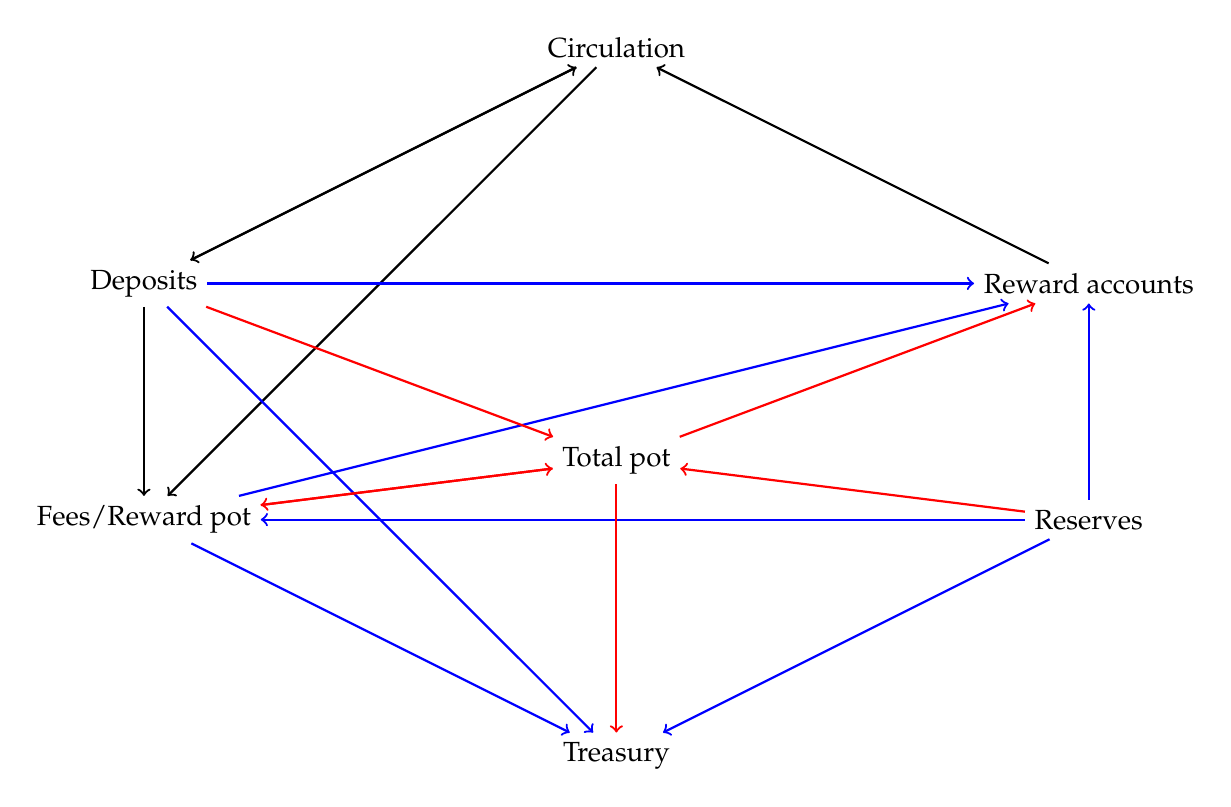
\begin{tikzpicture}
      [ x=30mm, y=30mm
      , direct/.style={black, draw}
      , implied/.style={blue, draw}
      , toTotPot/.style={red, draw}
      ]
    \node (C) at (3,3) {Circulation};
    \node (R) at (5, 1) {Reserves};
    \node (D) at (1, 2) {Deposits};
    \node (FR) at (1,1) {Fees/Reward pot};
    \node (RA) at (5, 2) {Reward accounts};
    \node (T) at (3,0) {Treasury};

    \draw[->, direct, thick]
    (C) edge (D)
    (C) edge (FR)

    (D) edge (C)
    (D) edge (FR)

    (RA) edge (C);

    \draw[->, implied, thick]
    (D) edge (RA)
    (D) edge (T)

    (FR) edge (T)
    (FR) edge (RA)

    (R) edge (FR)
    (R) edge (T)
    (R) edge (RA);

    \node (TP) at (3, 1.25) {Total pot};

    \draw[->, toTotPot, thick]
    (D) edge (TP)
    (FR) edge (TP)
    (R) edge (TP)

    (TP) edge (RA)
    (TP) edge (FR)
    (TP) edge (T);

  \end{tikzpicture}
  \end{center}
  \caption{Conservation of money}
  \label{fig:fund-preservation}
\end{figure}

%%
%% Figure - Functions for Epoch Rules
%%
\begin{figure}[htb]
  \emph{Total possible refunds}
  \begin{align*}
      & \fun{obligation} \in \PParams \to \StakeKeys \to \StakePools \to \Slot \to \Coin \\
      & \obligation{pp}{stkeys}{stpools}{cslot} =\\
      & \sum\limits_{(\_ \mapsto s) \in \var{stkeys}}
        \refund{d_{\mathsf{val}}}{d_{\min}}{\lambda_d}{(\slotminus{cslot}{s})}
        + \sum\limits_{(\_ \mapsto s) \in \var{stpools}}
        \refund{p_{\mathsf{val}}}{p_{\min}}{\lambda_p}{(\slotminus{cslot}{s})} \\
      &
      \begin{array}{lr@{~=~}l}
        \where
          & \dval,~d_{\min},~\lambda_d
          & \fun{keyDeposit}~\var{pp},~\fun{keyMinRefund}~\var{pp},~\fun{keyDecayRate}~\var{pp}
          \\
          & p_{\mathsf{val}},~p_{\min},~\lambda_p
          & \fun{poolDeposit}~\var{pp},~\fun{poolMinRefund}~\var{pp},~\fun{poolDecayRate}~\var{pp}
      \end{array}\\
  \end{align*}
  \emph{Pool refunds}
  \begin{align*}
      & \fun{poolRefunds} \in \PParams \to (\HashKey \mapsto \Epoch) \to \Slot \to 
        (\HashKey \mapsto \Coin) \\
      & \poolRefunds{pp}{retiring}{cslot} = \left\{
        \var{hk}\mapsto
          \refund{p_{\mathsf{val}}}{p_{\min}}{\lambda}{(\slotminus{cslot}{(\fun{slot}~e)})}
          \mid
          \var{hk}\mapsto e\in\var{retiring}
        \right\}\\
      & \where p_{\mathsf{val}},~p_{\min},~\lambda_p =
          \fun{poolDeposit}~\var{pp},~\fun{poolMinRefund}~\var{pp},~\fun{poolDecayRate}~\var{pp} \\
  \end{align*}

  \emph{Update Moving Averages}
  \begin{align*}
      & \fun{updateAvgs} \in \PParams \to \Avgs \to \BlocksMade \to
          (\HashKey_{pool}\mapsto \Stake) \to \Avgs \\
      & \updateAvgs{pp}{avgs}{blocks}{pooledStake} = \\
      & ~~~ \left\{hk\mapsto \movingAvg{pp}{hk}{n}{\overline{N}}{avgs}
            \mid
            hk\mapsto n\in\var{blocks}, hk\mapsto\overline{N}\in\var{expectations}
            \right\} \\
      & \where \\
      & ~~~~~ \var{tot} = \sum_{\_\mapsto st\in \var{pooledStake}}
                          \left(\sum_{\wcard\mapsto c\in\var{st}}c\right) \\
      & ~~~~~ \var{expectations} =
                \left\{
                  hk\mapsto\left(\sum_{\wcard\mapsto c\in\var{st}}c\right)*\slotsPer / tot
                  \mid
                  hk\mapsto\var{st} \in pooledStake
                \right\}
  \end{align*}
  \caption{Functions used in Accounting}
  \label{fig:functions:epoch}
\end{figure}

%%
%% Figure - Accounting Rules
%%
\begin{figure}[htb]
  \begin{equation}\label{eq:accnt}
    \inference[Accounting]
    {
      {
      \begin{array}{r@{=}l}
        \var{obl} & \obligation{pp}{stkeys}{stpools}{slot} \\
        \var{decayed} & \var{deposits} - \var{obl} \\
        \var{expansion} & \floor*{(\fun{rho}~{pp}) \cdot \var{reserves}} \\
        \var{totalPool} & \var{fees} + \var{decayed} + \var{rewardPot} + \var{expansion} \\
        \var{newTreasury} & \floor*{(\fun{tau}~{pp}) \cdot \var{totalPool}} \\
        \var{availablePool} & \var{totalPool} - \var{newTreasury} \\
        \var{pooledStake} & \poolDistr{utxo}{dstate}{pstate} \\
        \var{rewards'},~\var{unrealized} & \reward{pp}{blocks}{availablePool}{dpstate}{pooledStake}\\
        \var{newTreasury'} & \var{newTreasury} + \var{unrealized} \\
        \var{paidRewards} & \sum\limits_{\_\mapsto c\in\var{rewards'}}c \\
        \var{avgs'} & \updateAvgs{pp}{avgs}{blocks}{pooledStake} = \\
      \end{array}
      }
    }
    {
      \begin{array}{l}
        \var{slot}\\
        \var{pp}\\
        \var{blocks}\\
      \end{array}
      \vdash
      \left(
        \begin{array}{r}
          \var{treasury} \\
          \var{reserves} \\
          \var{rewardPot} \\
          \var{stkeys} \\
          \var{rewards} \\
          \var{delegations} \\
          \var{ptrs} \\
          \var{stpools} \\
          \var{poolParams} \\
          \var{retiring} \\
          \var{avgs} \\
          \var{utxo} \\
          \var{deposits} \\
          \var{fees} \\
        \end{array}
      \right)
      \trans{accnt}{}
      \left(
        \begin{array}{rcl}
          \varUpdate{\var{treasury}} & \varUpdate{+} & \varUpdate{\var{newTreasury'}} \\
          \varUpdate{\var{reserves}} & \varUpdate{-} & \varUpdate{\var{expansion}} \\
          \varUpdate{\var{availablePool}} & \varUpdate{-} & \varUpdate{\var{paidRewards}} \\
          \var{stkeys} \\
          \varUpdate{\var{rewards}} & \varUpdate{\unionoverridePlus} & \varUpdate{\var{rewards'}} \\
          \var{delegations} \\
          \var{ptrs} \\
          \var{stpools} \\
          \var{poolParams} \\
          \var{retiring} \\
          \varUpdate{\var{avgs'}} \\
          \var{utxo} \\
          \varUpdate{obl} \\
          \varUpdate{0} \\
        \end{array}
      \right)
    }
  \end{equation}
  \caption{Accounting Epoch inference rules}
  \label{fig:rules:accnt}
\end{figure}

\subsection{Epoch Boundary Pool Cleanup}
\label{sec:pool-clean}

Next, we discuss the epoch boundary pool retirement in
Figure~\ref{fig:ts-types:pool-clean}. The type of this transition is similar
to the other $\PState$ transition type we defined earlier, which is triggered
by a signal certificate,
however, this one has an empty signal (as it happens at the boundary).

%%
%% Figure - Pool Clean Defs
%%
\begin{figure}[htb]
  \begin{equation*}
    \_ \vdash \_ \trans{poolclean}{} \_ \in
    \powerset (\Slot \times \PState \times \PState)
  \end{equation*}
  %
  \caption{Pool Clean Transition}
  \label{fig:ts-types:pool-clean}
\end{figure}


We now present the pool-cleanup transition rule in Figure~\ref{fig:rules:pool-clean}.
This rule will be applied whenever there is one or more stake pools scheduled
to retire this epoch. If so, all of the entries in $\var{stpools}$,
$\var{poolParams}$, and $\var{retiring}$ which correspond to any of the hash keys
of the stake pools scheduled to retire this epoch are removed from
these variables.

It is important to note here that we \textit{do not} clean up delegations to
retired stake pools. While we do not allow registration to non-existent
stake pools (because that is a meaningless operation likely to be the result
of an error), delegating to a pool that was once active means that there may
be stake associated with this delegation. While this stake becomes inactive when
the pool is retired, the delegations to that pool must remain on the ledger
for potential future use.

%%
%% Figure - Pool Clean Rule
%%
\begin{figure}[htb]
  \begin{equation}\label{eq:pool-clean}
    \inference[Pool-Clean]
    {
      \var{retired} = \var{retiring}^{-1}~\var{(\epoch{slot})}
    }
    {
      \begin{array}{l}
        \var{slot}\\
      \end{array}
      \vdash
      \left(
        \begin{array}{r}
          \var{stpools} \\
          \var{poolParams} \\
          \var{retiring} \\
          \var{avgs} \\
        \end{array}
      \right)
      \trans{poolclean}{}
      \left(
        \begin{array}{rcl}
          \varUpdate{\var{retired}} & \varUpdate{\subtractdom} & \varUpdate{\var{stpools}} \\
          \varUpdate{\var{retired}} & \varUpdate{\subtractdom} & \varUpdate{\var{poolParams}} \\
          \varUpdate{\var{retired}} & \varUpdate{\subtractdom} & \varUpdate{\var{retiring}} \\
          \varUpdate{\var{retired}} & \varUpdate{\subtractdom} & \varUpdate{\var{avgs}} \\
        \end{array}
      \right)
    }
  \end{equation}
  \caption{Pool Clean Inference Rule}
  \label{fig:rules:pool-clean}
\end{figure}

\subsection{Epoch Boundary Protocol Constants Update}
\label{sec:prot-const-epoch}

Finally, reaching the epoch boundary may trigger a change in the protocol
parameters. Besides the current slot number, delegation and pool states, the
protocol constant environment includes the old and new protocol parameters.
The state change is a change of the $\UTxOState$ and the $\Accnt$ states.
The type of this state transition is given in Figure~\ref{fig:ts-types:new-proto-consts}.

%%
%% Figure - New Proto Consts Defs
%%
\begin{figure}[htb]
  \emph{New Proto Consts environment}
  \begin{equation*}
    \NewProtoConstsEnv =
    \left(
      \begin{array}{r@{~\in~}ll}
        \var{slot} & \Slot & \text{current slot}\\
        \var{ppOld} & \PParams & \text{old protocol parameters}\\
        \var{ppNew} & \PParams & \text{new protocol parameters}\\
        \var{dstate} & \DState & \text{delegation state}\\
        \var{pstate} & \PState & \text{pool state}\\
      \end{array}
    \right)
  \end{equation*}
  %
  \emph{New Proto Consts States}
  \begin{equation*}
    \NewProtoConstsState =
    \left(
      \begin{array}{r@{~\in~}ll}
        \var{utxoSt} & \UTxOState & \text{utxo state}\\
        \var{accnt} & \Accnt & \text{accounting}\\
      \end{array}
    \right)
  \end{equation*}
  %
  \emph{New Proto Consts transitions}
  \begin{equation*}
    \_ \vdash
    \var{\_} \trans{newpc}{} \var{\_}
    \subseteq \powerset (\NewProtoConstsEnv \times
    \NewProtoConstsState \times \NewProtoConstsState)
  \end{equation*}
  %
  \caption{New Proto Consts transition-system types}
  \label{fig:ts-types:new-proto-consts}
\end{figure}


The inference rule for changing protocol parameters does one of the following:

\begin{itemize}
\item if there are more (or the same amount of) total possible refunds
available calculated based on the old protocol parameters than the new ones,
moves the difference between the two values into the $\var{reserves}$
from the $\var{deposits}$ variable, \textit{or}

\item if there are more refunds available based on the new parameters, it moves
the difference between the two calculations from $\var{deposits}$
to $\var{reserves}$, \textit{provided that} there is enough coin in the
$\var{reserves}$ to cover the entire value of the transfer

\item if there are more refunds available based on the new parameters,
but there is \textit{not} enough coin in the $\var{reserves}$ to cover
the entire value of the transfer, the update is ignored entirely.
\end{itemize}

This update of protocol parameters ensures that any time a deposit refund is
requested, the necessary amount of funds is available in the $\var{deposits}$
pool.

Note that here, unlike most of the inference rules in this document,
the $\var{utxoSt'}$ and the $\var{accnt'}$ do not come from valid UTxO or
accounts transitions in the antecedent. We simply define the consequent
transition using these directly (instead of listing all the fields in both
states in the consequent transition). It is done this way here
for ease of reading.

%%
%% Figure - New Proto Consts Rule
%%
\begin{figure}[htb]
  \begin{equation}\label{eq:new-pc-accepted}
    \inference[New-Proto-Consts-Accepted]
    {
      \var{oblgOld} = \obligation{ppOld}{stkeys}{stpools}{slot} \\
      \var{oblgNew} = \obligation{ppNew}{stkeys}{stpools}{slot} \\
      ~\\
      \var{diff} = \var{oblgOld} - \var{oblgNew} \\
      \var{reserves} + \var{diff} \geq 0\\
      ~\\
      \var{utxoSt'} =
      \left(
        {
          \begin{array}{r}
            \var{utxo} \\
            \varUpdate{oblgNew} \\
            \var{fees} \\
          \end{array}
        }
      \right)
      &
      \var{accnt'} =
      \left(
        {
          \begin{array}{r}
            \var{treasury} \\
            \varUpdate{reserves + diff} \\
            \var{rewardPot} \\
            \var{rewards} \\
          \end{array}
        }
      \right)
    }
    {
      \begin{array}{l}
        \var{slot}\\
        \var{ppOld}\\
        \var{ppNew}\\
        \var{dstate}\\
        \var{pstate}\\
      \end{array}
      \vdash
      \left(
        \begin{array}{r}
          \var{utxoSt} \\
          \var{accnt}
        \end{array}
      \right)
      \trans{newpc}{}
      \left(
        \begin{array}{rcl}
          \varUpdate{utxoSt'}\\
          \varUpdate{accnt'} \\
        \end{array}
      \right)
    }
  \end{equation}

  \nextdef

  \begin{equation}\label{eq:new-pc-denied}
    \inference[New-Proto-Consts-Denied]
    {
      \var{oblgOld} = \obligation{ppOld}{stkeys}{stpools}{slot} \\
      \var{oblgNew} = \obligation{ppNew}{stkeys}{stpools}{slot} \\
      ~\\
      \var{diff} = \var{oblgOld} - \var{oblgNew} \\
      \var{reserves} + \var{diff} < 0\\
    }
    {
      \begin{array}{l}
        \var{slot}\\
        \var{ppOld}\\
        \var{ppNew}\\
        \var{dstate}\\
        \var{pstate}\\
      \end{array}
      \vdash
      \left(
        \begin{array}{r}
          \var{utxoSt} \\
          \var{accnt}
        \end{array}
      \right)
      \trans{newpc}{}
      \left(
        \begin{array}{rcl}
          \var{utxoSt} \\
          \var{accnt}
        \end{array}
      \right)
    }
  \end{equation}
  \caption{New Proto Consts Inference Rule}
  \label{fig:rules:new-proto-consts}
\end{figure}

\subsection{Complete Epoch Boundary Transition}
\label{sec:total-epoch}

Finally, it is possible to define the complete epoch boundary transition type.
In the environment of this transition, we have the slot number, blocks made
this epoch, and both the old and the new protocol parameters. The state is
made up of the accounting state, the UTxO, the delegation state and the
pool state.

%%
%% Figure - Epoch Defs
%%
\begin{figure}[htb]
  \emph{Epoch environment}
  \begin{equation*}
    \EpochEnv =
    \left(
      \begin{array}{r@{~\in~}ll}
        \var{slot} & \Slot & \text{current slot}\\
        \var{ppOld} & \PParams & \text{old protocol parameters}\\
        \var{ppNew} & \PParams & \text{new protocol parameters}\\
        \var{blocks} & \HashKey \mapsto \N & \text{blocks made in the epoch}\\
      \end{array}
    \right)
  \end{equation*}
  %
  \emph{Epoch States}
  \begin{equation*}
    \EpochState =
    \left(
      \begin{array}{r@{~\in~}ll}
        \var{utxoSt} & \UTxOState & \text{utxo state}\\
        \var{accnt} & \Accnt & \text{accounting}\\
        \var{dstate} & \DState & \text{delegation state}\\
        \var{pstate} & \PState & \text{pool state}\\
      \end{array}
    \right)
  \end{equation*}
  %
  \emph{Epoch transitions}
  \begin{equation*}
    \_ \vdash
    \var{\_} \trans{epoch}{} \var{\_}
    \subseteq \powerset (\EpochEnv \times \EpochState \times \EpochState)
  \end{equation*}
  %
  \caption{Epoch transition-system types}
  \label{fig:ts-types:epoch}
\end{figure}


The epoch transition rule is a composition of all the state transition rules
we have defined above. That is, whenever the UTXOEP, ACCNT, POOLCLEAN, and
NEWPC are all valid transitions between their respective pairs of sets of
state variables, the total transition epoch boundary ledger state transition
is a composition of these four rules in that order.

Note that the slot number used as \textit{current slot number}
for the epoch boundary calculations where a slot number is required is set to
be the \textit{last slot of the epoch before the boundary}.

%%
%% Figure - Epoch Rule
%%
\begin{figure}[htb]
  \begin{equation}\label{eq:epoch}
    \inference[Epoch]
    {
      {
        \begin{array}{l}
          \var{slot}\\
          \var{ppOld}\\
          \var{blocks}\\
        \end{array}
      }
      \vdash
      \left(
        {
          \begin{array}{r}
            \var{accnt} \\
            \var{dstate} \\
            \var{pstate} \\
            \var{utxoSt} \\
          \end{array}
        }
      \right)
      \trans{accnt}{}
      \left(
      {
        \begin{array}{rcl}
          \var{accnt'} \\
          \var{dstate'} \\
          \var{pstate'} \\
          \var{utxoSt'} \\
        \end{array}
      }
      \right)
      \\~\\~\\
      {
        \begin{array}{l}
          \var{slot}
        \end{array}
      }
      \vdash
      \left(
        {
          \begin{array}{r}
            \var{pstate'} \\
          \end{array}
        }
      \right)
      \trans{poolclean}{}
      \left(
      {
        \begin{array}{rcl}
            \var{pstate''} \\
        \end{array}
      }
      \right)
      \\~\\~\\
      {
        \begin{array}{l}
          \var{slot}\\
          \var{ppOld}\\
          \var{ppNew}\\
          \var{dstate'}\\
          \var{pstate''}\\
        \end{array}
      }
      \vdash
      \left(
        {
          \begin{array}{r}
            \var{utxoSt'} \\
            \var{accnt'} \\
          \end{array}
        }
      \right)
      \trans{newpc}{}
      \left(
      {
        \begin{array}{rcl}
            \var{utxoSt''} \\
            \var{accnt''} \\
        \end{array}
      }
      \right)
    }
    {
      \begin{array}{l}
        \var{slot}\\
        \var{ppOld}\\
        \var{ppNew}\\
        \var{blocks}\\
      \end{array}
      \vdash
      \left(
      \begin{array}{r}
        \var{utxoSt} \\
        \var{accnt} \\
        \var{dstate} \\
        \var{pstate}
      \end{array}
      \right)
      \trans{epoch}{}
      \left(
      \begin{array}{rcl}
        \varUpdate{\var{utxoSt''}} \\
        \varUpdate{\var{accnt''}} \\
        \varUpdate{\var{dstate'}} \\
        \varUpdate{\var{pstate''}}
      \end{array}
      \right)
    }
  \end{equation}
  \caption{Epoch Inference Rule}
  \label{fig:rules:epoch}
\end{figure}


\clearpage

\section{Properties}
\label{sec:properties}


\input{properties}

\addcontentsline{toc}{section}{References}
\bibliographystyle{plainnat}
\bibliography{references}

\end{document}
